% !Mode:: "TeX:UTF-8"
%!TEX program  = xelatex

% \documentclass{cumcmthesis}
\documentclass[withoutpreface,bwprint]{cumcmthesis} %去掉封面与编号页
\usepackage{multirow}
\usepackage{url}
\usepackage{enumitem}
\usepackage{tikz}
\usepackage{xcolor}
\usepackage{graphicx} % 图片插入需要的宏包
\usepackage{float}
\usepackage{subcaption}
\usepackage{zhlipsum,mwe}
\usepackage{mathrsfs}
\usepackage{multirow}
% \usepackage{floatrow}
\usepackage{tikz}
\usepackage{booktabs}
\usepackage{threeparttable}
\usepackage{adjustbox}
% \usepackage{floatrow}
\usepackage{xcolor}
\usepackage{wrapfig}
\usepackage{longtable}
\usepackage{hyperref}
\usepackage{cleveref}
\usepackage[linesnumbered,ruled,vlined]{algorithm2e}
\SetKwInput{KwIn}{输入} 
\SetKwInput{KwOut}{输出}
\renewcommand{\algorithmcfname}{算法}


\crefname{equation}{式}{式}
\Crefname{equation}{式}{式}
\lstset{ 
  backgroundcolor=\color{white},   				% 选择代码背景,必须加上\usepackage{color}或\usepackage{xcolor}.
  basicstyle=\footnotesize,        				% 设置代码字号.
  breakatwhitespace=false,        				% 设置是否当且仅当在空白处自动中断.
  breaklines=true,                				% 设置自动断行.
  captionpos=b,                    				% 设置标题位置.
  commentstyle=\color{green},    				% 设置注释格式
  deletekeywords={...},           				% 是否删除给定语言的关键词.
  escapeinside={\%*}{*)},          				% 是否在代码中添加LaTex. 
  frame=single,	                   				% 给代码区添加边框.
  keepspaces=true,                 				% 保留空格(useful for keeping indentation of code (possibly needs columns=flexible).
  keywordstyle=\color[RGB]{40,40,255},          % 关键字显示风格.
  morekeywords={begin}, 			% 是否需要添加其他关键词
  numbers=none,                    				% 给代码添加行号,可取值none, left, right.
  numbersep=5pt,                   				% 设置行号与代码之间的间隔
  numberstyle=\tiny\color{gray}, 				% 行号的字号和颜色
  rulecolor=\color{black},         				% 边框颜色,如果没有设置,框架颜色可以在非黑色文本中的换行符上更改(例如 text (e.g. comments (green here)))
  showspaces=false,                				% 显示每个地方添加特定下划线的空格; 覆盖了'showtringspaces'
  showstringspaces=false,          				% 仅在字符串中允许空格
  showtabs=false,                  				% show tabs within strings adding particular underscores
  stepnumber=2,                    				% the step between two line-numbers. If it's 1, each line will be numbered
  stringstyle=\color{teal},     				% string literal style
  tabsize=2,	                   				% 将默认tab设置为2个空格
  title=\lstname,                  	 			% show the filename of files included with \lstinputlisting; also try caption instead of title
  language=Matlab
}
\usetikzlibrary{patterns}
\title{基于SolarPILOT软件的定日镜场优化问题}


\begin{document}

\maketitle
 \begin{abstract}
本文在优化定日镜场最大平均单位镜面面积输出功率设计中,建立了镜面坐标系、太阳光锥坐标系,并计算得到其与镜场坐标系间的转换关系矩阵,利用随机化模拟方法,计算出了在定日镜场各参数已知的情况下的平均光学效率和输出功率等结果。同时对定日镜场结构进行优化后,利用SolarPILOT软件实现COBYLA算法对定日镜场的输出功率优化,通过移除输出功率较低的定日镜得到在优化后的镜场各参数值使得在达到额定功率情况下单位面积镜面面积年平均输出热功率尽量大。并对本文模型和算法进行了检验和评价。

\textbf{针对问题一:}本文首先建立了镜面坐标系用于余弦效率和阴影遮挡效率的计算中,通过各坐标系间的转换关系矩阵以及入射光、反射光和法线间的数量关系得到余弦角进而计算余弦效率。其次,利用蒙特卡洛模拟方法计算得到了各镜面的阴影遮挡效率。再进一步,建立了太阳光锥坐标系用于求解截断效率,利用蒙特卡洛光际追踪算法,计算得到了各镜面的截断效率。最后,利用题中所给公式得到年平均光学效率及输出功率(见下表)和每月21日的平均光学效率及输出功率(详见表\ref{a1})。
\noindent
\resizebox{\textwidth}{!}{
\begin{tabular}{@{}lccccc@{}}
\toprule
\textbf{年平均光学效率}     & \textbf{年平均余弦效率}  & \textbf{年平均阴影遮挡效率}   & \textbf{年平均截断效率}    & \textbf{年平均输出热功率 ($MW$)} & \textbf{单位面积镜面年平均输出热功率 ($kW/m^2$)} \\ \midrule
\textbf{0.546718499} & \textbf{0.759902} & \textbf{0.987169083} & \textbf{0.82211874} & \textbf{33.382548}       & \textbf{0.5314}                    \\ \bottomrule
\end{tabular}}

\textbf{针对问题二:}考虑到镜场布局较为疏松,首先使用DELSOL3布局对定日镜场的布局进行优化,再利用SolarPILOT软件中的COBYLA算法对镜场输出功率进行仿真优化。在这里可优化的镜场参数为定日镜分布情况,定日镜镜面高度、宽度、安装高度以及吸收塔位置,优化后得到在满足约束条件的情况下月平均光学效率、输出功率(详见表\ref{s1}),年平均光学效率、输出功率以及镜场设计参数表(见下表)。

\noindent
\resizebox{\textwidth}{!}{
\begin{tabular}{@{}cccccc@{}}
\toprule
\textbf{年平均光学效率}     & \textbf{年平均余弦效率}  & \textbf{年平均阴影遮挡效率}   & \textbf{年平均截断效率}    & \textbf{年平均输出热功率 ($MW$)} & \textbf{单位面积镜面年平均输出热功率 ($kW/m^2$)} \\ \midrule
\textbf{0.546718499} & \textbf{0.759902} & \textbf{0.987169083} & \textbf{0.82211874} & \textbf{33.382548}       & \textbf{0.5314}                    \\ \bottomrule
\end{tabular}}
\noindent
\resizebox{\textwidth}{!}{
\begin{tabular}{@{}ccccc@{}}
\toprule
\textbf{吸收塔位置坐标}        & \textbf{定日镜尺寸(宽 ×高)} & \textbf{定日镜安装高度(m)} & \textbf{定日镜总面数} & \textbf{定日镜总面积($m^2$)} \\ \midrule
$\mathbf{(4.52465\times10^{-7},0)}$ & \textbf{7.3×6.1}     & \textbf{6}        & \textbf{2233}   & \textbf{99435.49}      \\ \bottomrule
\end{tabular}}

\textbf{针对问题三:}基于问题二的求解过程,使用SolarPILOT软件将镜场分为50个不同半径的同心圆环区域,对各区域定日镜的镜面宽度和高度以及安装高度进行仿真优化,最终进行整合得到定日镜场的各项设计参数以及月平均光学效率、输出功率,年平均光学效率、输出功率。

\par
\keywords{蒙特卡洛模拟\quad 光际追踪法\quad SolorPILOT软件}
\end{abstract}

%目录
% \tableofcontents



%  %图片
% \begin{figure}[H]
% \centering
% 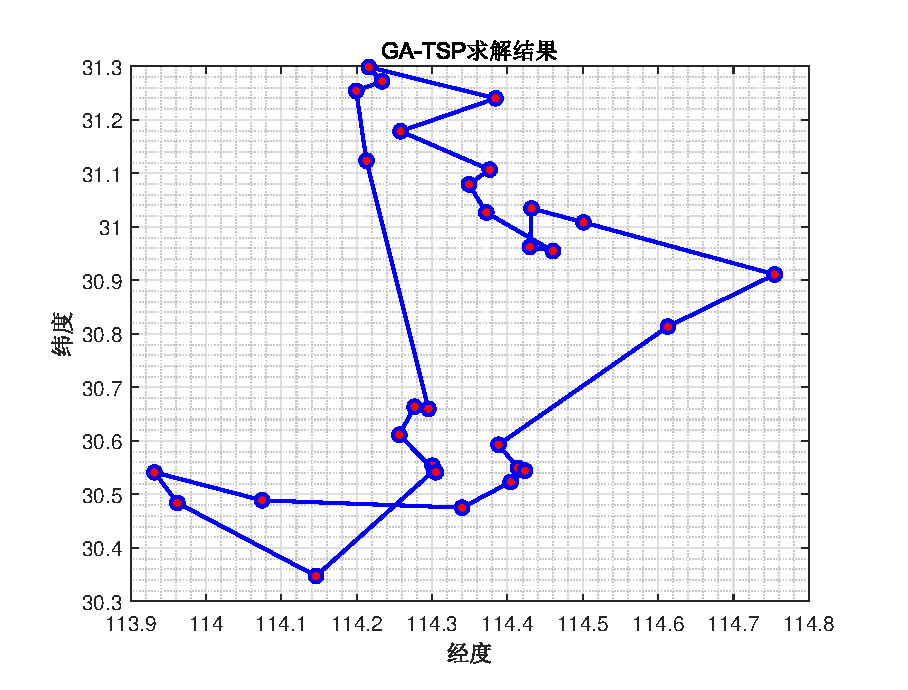
\includegraphics[scale=0.95]{figures/a.eps}
% \caption{最短时间路径示意图}
% \end{figure}
% \begin{eqnarray}
% \mathbf{V}|_{H_B}=\mathbf{T_B}^{-1}\cdot \mathbf{V}|_{H_0}
% \end{eqnarray}



































































\section{问题重述}
\subsection{问题背景}
近年来,随着社会的发展,人类对能源的依赖和消耗越来越大,塔式太阳能发电是一种具有广阔发展前景的太阳能发电技术,如何更好的安排定日镜的位置,面积大小,各定日镜间距离等,都直接影响到定日镜场的年平均光学效率和输出热功率。

\textbf{镜场组成:}定日镜场主要由定日镜和中心的吸收塔组成,各定日镜可以根据太阳光调节法向,具有跟踪和聚光两大功能,在结构上主要分为底座以及聚光镜面。在吸收塔上存在圆柱形外表受光式集热器。

\textbf{镜场参数:}镜场参数主要分为定日镜参数和集热器参数。其中定日镜参数有定日镜宽度,定日镜高度,定日镜底座高度,定日镜数量,定日器中心位置;集热器参数有集热器高度,集热器直径以及底部吸收塔高度。
\subsection{问题重述}


问题一:给出定日镜的尺寸及安装的空间位置,根据附录中所给公式计算该定日镜场的年平均光学效率、年平均输出热功率以及单位镜面面积平均输出热功率,并将结果填入表格。

问题二:在满足定日镜场额定年平均为60MW以及所有定日镜尺寸和安装高度相同情况下,设计定日镜场参数使得在达到额定功率条件下,使得单位镜面面积年平均输出功率尽量大,并将相关结果填入表格或附件。

问题三:在问题二基础上,允许定日镜尺寸和安装高度可以不同,重新设计定日镜场各参数,并将相关结果填入表格或附件。
\section{模型假设}
\begin{itemize}
	\item 太阳光并非平行光线, 而是具有一定锥形角的一束锥形光线。
	\item 为简化计算,年均指标的计算时间点为题目所给的60个时间点。
	\item 所有定心镜的前后两侧在地面的投影均与从该定心镜的中心指向整个镜场中心的连线垂直。
	\item 在计算中近似认为相邻定心镜镜面间相互平行。
	\item 在计算阴影遮挡效率时不考虑三个遮挡损失存在重叠部分。
	\item 不考虑天气对定日镜场的影响。
	\item 认为地形平坦,不存在除定日镜和吸收塔之外的遮挡物。
\end{itemize}
\section{符号说明}
\begin{longtable}[c]{@{}ccl@{}}
\toprule
序号 & 符号  & 符号说明 \\* \midrule
\endfirsthead
%
\multicolumn{3}{c}%
{{\bfseries 表\thetable (续)}} \\
\toprule
序号 & 符号  & 符号说明 \\* \midrule
\endhead
%
1  & $H_0$ & 镜场坐标系  \\
2  & $H_i$ & 镜面$i$坐标系  \\
3  & $H_s$ & 太阳光锥坐标系  \\
4  & $H|_{H_i}$ & 点$H$在坐标系$H_i$下的坐标表示 \\
5&$\mathbf{V}|_{H_i}$&向量$\mathbf{V}$在坐标系$H_i$下的坐标表示\\
6&$\mathbf{T_i}$&坐标系$H_i$转换到坐标系$H_0$的转换关系矩阵\\ 
7&$\mathbf{T_S}$&从坐标系$H_s$转换到坐标系$H_0$的转换关系矩阵\\ 
8&$O_i$&定心镜$i$中心坐标\\ 
9&$EH_i$&坐标系$H_i$中$Z_i$轴与坐标系$H_0$中$Z$轴夹角\\ 
10&$AH_i$&坐标系$H_i$中$Y_i$轴在镜场坐标系$XOY$平面投影与$X$轴夹角\\ 
11&$\mathbf{i}$&太阳光入射方向的单位向量\\ 
12&$\mathbf{R}$&经平面镜反射向量\\ 
13&$J$&坐标系$H_0$下集热器方程\\ 
14&$\hat{E}$&单位镜面面积输出热功率\\
15&$LH$&定日镜宽高\\ 
16&$LW$&定日镜高度\\ 
17&$RH$&定日镜安装高度\\ 
18&$DM$&定日镜中心间距离\\ 
19&$DH$&定日镜镜面对角线长度\\ 
20&$\Delta R_h$&相邻行间之间的最小增量 \\ 
21&$\Delta R_f$&相邻区域之间的最小增量\\ 
22&$n$&基本区域数量\\
23&$N$&第一行定日镜数量\\* \bottomrule
\end{longtable}

\section{问题分析}
\subsection{问题一分析}
对于问题一,问题所要求数据均不能通过简单计算得到,我们需要通过建立模型进行求解。其中需要注意的是我们要求的值分布在12个月的21号的5个时间点,我们需要对这60个时间分别进行求解。

对于平均遮挡效率,我们可以建立镜面坐标系,通过计算得到镜面坐标系和镜场坐标系的转换关系矩阵。以镜面A的遮挡效率计算为例,将被遮挡面积分为三个部分:入射光线被遮挡,反射光线被遮挡以及吸收塔对其的遮挡。我们分别进行分析:

对于入射光线被遮挡情况,以镜面B对其遮挡为例:考虑将镜面B坐标转换到镜面A坐标系下计算其遮挡面积,由于其投影形状可能并不规则,可以考虑随机化算法例如蒙特卡洛模拟算法,在模拟点足够多情况下,落在镜面A上点的数量与总模拟点的比值等于镜面B在镜面A上的遮挡面积占比。
对于反射光线被遮挡情况,以镜面B对其遮挡为例:根据镜面A入射向量和法向量计算其反射向量,将镜面A坐标转换到镜面B坐标系下计算其遮挡面积,也可以通过蒙特卡洛模拟算法求解其反射光线被镜面B遮挡面积占比。
对于被吸收塔遮挡的情况,同理利用蒙特卡洛算法,计算经过吸收塔内任一点的光线是否落入镜面A内,可求解得到被吸收塔遮挡面积占比。
将以上三种情况遮挡面积占比相加,不考虑三种情况存在遮挡面积重叠情况下近似认为等于计算得到被遮挡面积占比等于实际情况。

对于平均余弦效率,我们已知太阳光入射向量和镜面反射向量,根据入射向量、反射向量和法线向量间关系,计算得到反射向量,根据题目所给公式计算各镜面余弦效率。
对于平均截断效率,考虑太阳光为一束光锥情况下,建立光锥坐标系,利用蒙特卡洛光际追踪法,判断经定日镜反射后光线是否落在集热器上并根据其总占比进而计算各镜面截断效率。
得到遮挡效率、余弦效率、截断效率后进而带入题目所给公式计算所要求结果。
\subsection{问题二分析}
在问题二中,要求我们设计定日镜场中部分参数,包括吸收塔的位置坐标、定日镜尺寸、安装高度、定日镜数目、定日镜位置,使得达到额定功率情况下优化单位面积镜面平均输出热功率。考虑在问题一中定日镜场排布较为稀疏,没有达到较高的面积利用率,我们可以先对定日镜场布局进行优化,使得在阴影遮挡损失效率较高的情况下,提高土地利用率。本文考虑 DELSOL3 布局,可优化的参数为定日镜尺寸及安装高度。考虑将优化后的镜场坐标输入仿真软件进行优化。运用SolarPILOT 软件,在该问已知参数情况下,能够得出最优的镜场单位镜面面积年平均输出功率,首先我们取定定日镜长宽高度、中心间距以及吸收塔的位置的优化范围,并设置步长,得出符合额定功率要求的定日镜参数,并选取最优参数,然后逐渐缩小步长,进行多次迭代,找出符合条件的最优解。
\subsection{问题三分析}
在问题三中,我们将镜场由内到外划分为50个不同半径的同心圆环区域,在各区域内各自对定日镜的长宽高度进行约束优化,与问题二的处理方法相似,进行多次迭代后,我们可以得出每一个区域的最优长宽高数值。最终将所有数据整合在一张图中,对各区域定日镜的高度进行整合排布,细化处理。最终将阴影遮挡效率、余弦效率和截断效率等数据导出并计算,得出最后结论。





















% \begin{eqnarray}
% a^2+b^2=c^2\label{key}
% \end{eqnarray}

% 见式\eqref{key}

% 高德API$^\text{\cite{noauthor_---js_nodate}}$


\section{问题一模型建立与求解}
\subsection{基本数据的求解}
本题中许多数据都已给出相关计算公式,按条件求解即可。值得注意的是需要求解每个月份的21号的五个时间点进行求解,即太阳高度角$\alpha_s$、方位角$\gamma_s$、时角$\omega$、赤纬角$\delta _s$、法向直接辐射强度(DNI)等数据均需要求解60个不用时间点的值。其中部分数据见表\ref{a0}:
\begin{table}[H]
\centering
\caption{部分数据结果展示}
\label{a0}\resizebox{\textwidth}{!}{
\begin{tabular}{@{}cccccccc@{}}
\toprule
\textbf{D} & \textbf{ST} & \textbf{太阳时角} & \textbf{定日镜位置} & \textbf{太阳方位角} & \textbf{太阳高度角} & \textbf{赤纬角} & \textbf{DNI} \\ \midrule
-59 & 9    & -0.7854 & (107.25,11.664)    & -0.71661 & 0.2996 & -0.3382 & 0.7925397 \\
31  & 9    & -0.7854 & (-12.697,-161.325) & -0.37844 & 0.6636 & 0.2024  & 0.9992775 \\
61  & 10.5 & -0.3927 & (-25.41,227.837)   & -0.61974 & 0.8891 & 0.3452  & 1.0572471 \\
122 & 10.5 & 0.3927  & (-209.77,147.124)  & -0.62176 & 0.8885 & 0.3435  & 1.0571177 \\
214 & 13.5 & 0.3927  & (-248,136.722)     & -0.89039 & 0.5683 & -0.2054 & 0.9642047 \\ \bottomrule
\end{tabular}}
\end{table}

% \subsection{定日镜光学效率模型建立}
\subsection*{镜面坐标系的建立}
我们以镜面$i$为例,以镜面中心$O_i$为坐标原点,沿镜面长方向为$X_i$轴,宽方向为$Y_i$轴,垂直镜面方向向上为$Z_i$轴,建立镜面$i$坐标系,如图\ref{j1}所示:$^\text{\cite{x}\cite{xx}}$

\begin{figure}[H]
\begin{center}
\tikzset{every picture/.style={line width=0.75pt}} %set default line width to 0.75pt        

\begin{tikzpicture}[x=0.75pt,y=0.75pt,yscale=-1,xscale=1]
%uncomment if require: \path (0,300); %set diagram left start at 0, and has height of 300

%Shape: Rectangle [id:dp0740170910478648] 
\draw   (141.37,122.44) -- (245.37,122.44) -- (245.37,212.04) -- (141.37,212.04) -- cycle ;
%Straight Lines [id:da934035686023001] 
\draw    (189.95,169.67) -- (318.51,169.36) ;
\draw [shift={(320.51,169.36)}, rotate = 179.86] [color={rgb, 255:red, 0; green, 0; blue, 0 }  ][line width=0.75]    (10.93,-3.29) .. controls (6.95,-1.4) and (3.31,-0.3) .. (0,0) .. controls (3.31,0.3) and (6.95,1.4) .. (10.93,3.29)   ;
%Straight Lines [id:da7321735429102307] 
\draw    (189.95,169.67) -- (190.03,67.9) ;
\draw [shift={(190.03,65.9)}, rotate = 90.04] [color={rgb, 255:red, 0; green, 0; blue, 0 }  ][line width=0.75]    (10.93,-3.29) .. controls (6.95,-1.4) and (3.31,-0.3) .. (0,0) .. controls (3.31,0.3) and (6.95,1.4) .. (10.93,3.29)   ;
%Straight Lines [id:da4875117934493709] 
\draw    (189.95,169.67) -- (121.69,228.54) ;
\draw [shift={(120.18,229.85)}, rotate = 319.22] [color={rgb, 255:red, 0; green, 0; blue, 0 }  ][line width=0.75]    (10.93,-3.29) .. controls (6.95,-1.4) and (3.31,-0.3) .. (0,0) .. controls (3.31,0.3) and (6.95,1.4) .. (10.93,3.29)   ;

% Text Node
\draw (299.6,171.8) node [anchor=north west][inner sep=0.75pt]   [align=left] {$\displaystyle X_{i}$};
% Text Node
\draw (192.8,66.2) node [anchor=north west][inner sep=0.75pt]   [align=left] {$\displaystyle Y_{i}$};
% Text Node
\draw (134.4,221) node [anchor=north west][inner sep=0.75pt]   [align=left] {$\displaystyle Z_{i}$};
% Text Node
\draw (191.95,172.67) node [anchor=north west][inner sep=0.75pt]   [align=left] {$\displaystyle O_{i}$};


\end{tikzpicture}
\end{center}
\caption{镜面$i$坐标系示意图}\label{j1}
\end{figure}

定义$H_0$表示镜场坐标系,$\mathbf{V}|_{H_k}$表示向量$\mathbf{V}$在坐标系$H_k$下的坐标表示,$H|_{H_k}$表示点$H$在坐标系$H_k$下的坐标表示。定日镜$i$的镜面中心在$H_0$下的坐标表示为$O_i|_{H_0}=(XgH_i,YgH_i,ZgH_i)$,镜面$i$坐标系$H_i$转换为镜场坐标系$H_0$的转换关系矩阵为$\mathbf{T_i}$,则有:

\begin{eqnarray}
\mathbf{V}|_{H_0}=\mathbf{T_i}\cdot \mathbf{V}|_{H_i}
\end{eqnarray}
\begin{eqnarray}
H|_{H_0}=\mathbf{T_i}\cdot H|_{H_i}+O_i|_{H_i}
\end{eqnarray}
\begin{eqnarray}
\mathbf{T_i}=\begin{bmatrix}
  -\sin AH_i&-\cos AH_i\cos EH_i  &\cos AH_i\sin EH_i \\
  \cos AH_i&-\sin AH_i\cos EH_i  &\sin AH_i\sin EH_i \\
  0&\sin EH_i  &\cos EH_i
\end{bmatrix}
\end{eqnarray}
其中,$EH_i$表示镜面$i$坐标系$Z_i$轴与镜场坐标系$Z$轴夹角,$AH_i$表示镜面$i$坐标系$Y_i$轴在镜场坐标系$XOY$平面投影与$X$轴夹角。如图\ref{i0}所示:

\begin{figure}[H]
\begin{center}


\tikzset{every picture/.style={line width=0.75pt}} %set default line width to 0.75pt        

\begin{tikzpicture}[x=0.75pt,y=0.75pt,yscale=-1,xscale=1]
%uncomment if require: \path (0,300); %set diagram left start at 0, and has height of 300

%Shape: Rectangle [id:dp5249850634512643] 
\draw   (158.47,97.66) -- (209.62,124.13) -- (187.41,170.11) -- (136.26,143.64) -- cycle ;
%Straight Lines [id:da6169596885747695] 
\draw    (170.65,134.26) -- (233.16,166.41) ;
\draw [shift={(234.94,167.32)}, rotate = 207.22] [color={rgb, 255:red, 0; green, 0; blue, 0 }  ][line width=0.75]    (10.93,-3.29) .. controls (6.95,-1.4) and (3.31,-0.3) .. (0,0) .. controls (3.31,0.3) and (6.95,1.4) .. (10.93,3.29)   ;
%Straight Lines [id:da6683895218009517] 
\draw    (170.65,134.26) -- (195.54,82.83) ;
\draw [shift={(196.41,81.03)}, rotate = 115.82] [color={rgb, 255:red, 0; green, 0; blue, 0 }  ][line width=0.75]    (10.93,-3.29) .. controls (6.95,-1.4) and (3.31,-0.3) .. (0,0) .. controls (3.31,0.3) and (6.95,1.4) .. (10.93,3.29)   ;
%Straight Lines [id:da9575843530740704] 
\draw    (170.65,134.26) -- (228.45,64.22) ;
\draw [shift={(229.72,62.68)}, rotate = 129.53] [color={rgb, 255:red, 0; green, 0; blue, 0 }  ][line width=0.75]    (10.93,-3.29) .. controls (6.95,-1.4) and (3.31,-0.3) .. (0,0) .. controls (3.31,0.3) and (6.95,1.4) .. (10.93,3.29)   ;
%Straight Lines [id:da70977854381131] 
\draw  [dash pattern={on 4.5pt off 4.5pt}]  (170.12,40.68) -- (170.08,161.07) ;
%Straight Lines [id:da5129481008433583] 
\draw    (170.88,197.47) -- (426.12,197.48) ;
\draw [shift={(428.12,197.48)}, rotate = 180] [color={rgb, 255:red, 0; green, 0; blue, 0 }  ][line width=0.75]    (10.93,-3.29) .. controls (6.95,-1.4) and (3.31,-0.3) .. (0,0) .. controls (3.31,0.3) and (6.95,1.4) .. (10.93,3.29)   ;
%Straight Lines [id:da11799820710609876] 
\draw    (376.12,207.88) -- (375.33,68.68) ;
\draw [shift={(375.32,66.68)}, rotate = 89.68] [color={rgb, 255:red, 0; green, 0; blue, 0 }  ][line width=0.75]    (10.93,-3.29) .. controls (6.95,-1.4) and (3.31,-0.3) .. (0,0) .. controls (3.31,0.3) and (6.95,1.4) .. (10.93,3.29)   ;
%Straight Lines [id:da14883900970595243] 
\draw    (376.52,197.48) -- (414.68,160.86) ;
\draw [shift={(416.12,159.48)}, rotate = 136.18] [color={rgb, 255:red, 0; green, 0; blue, 0 }  ][line width=0.75]    (10.93,-3.29) .. controls (6.95,-1.4) and (3.31,-0.3) .. (0,0) .. controls (3.31,0.3) and (6.95,1.4) .. (10.93,3.29)   ;
%Curve Lines [id:da8581353820474187] 
\draw    (172.98,74.59) .. controls (189.09,68.18) and (203.15,76.13) .. (210.01,82.23) ;
\draw [shift={(212.12,84.28)}, rotate = 226.85] [fill={rgb, 255:red, 0; green, 0; blue, 0 }  ][line width=0.08]  [draw opacity=0] (10.72,-5.15) -- (0,0) -- (10.72,5.15) -- (7.12,0) -- cycle    ;
\draw [shift={(170.12,75.88)}, rotate = 333.43] [fill={rgb, 255:red, 0; green, 0; blue, 0 }  ][line width=0.08]  [draw opacity=0] (10.72,-5.15) -- (0,0) -- (10.72,5.15) -- (7.12,0) -- cycle    ;
%Straight Lines [id:da9757663450855989] 
\draw    (170.08,161.07) -- (170.88,197.47) ;
%Straight Lines [id:da9027227130039683] 
\draw  [dash pattern={on 4.5pt off 4.5pt}]  (229.72,62.68) -- (230.12,155.88) ;
%Straight Lines [id:da47166094255056645] 
\draw  [dash pattern={on 4.5pt off 4.5pt}]  (170.88,197.47) -- (277.72,121.48) ;
%Curve Lines [id:da8440561725728954] 
\draw    (236.97,154.11) .. controls (254.65,161.54) and (256.6,182.63) .. (255.01,194.58) ;
\draw [shift={(254.52,197.48)}, rotate = 281.69] [fill={rgb, 255:red, 0; green, 0; blue, 0 }  ][line width=0.08]  [draw opacity=0] (10.72,-5.15) -- (0,0) -- (10.72,5.15) -- (7.12,0) -- cycle    ;
\draw [shift={(234.12,153.08)}, rotate = 17.18] [fill={rgb, 255:red, 0; green, 0; blue, 0 }  ][line width=0.08]  [draw opacity=0] (10.72,-5.15) -- (0,0) -- (10.72,5.15) -- (7.12,0) -- cycle    ;

% Text Node
\draw (215.82,160.49) node [anchor=north west][inner sep=0.75pt]  [rotate=-26.56] [align=left] {$\displaystyle X_{i}$};
% Text Node
\draw (196.86,84.6) node [anchor=north west][inner sep=0.75pt]  [rotate=-26.56] [align=left] {$\displaystyle Y_{i}$};
% Text Node
\draw (231.74,65.67) node [anchor=north west][inner sep=0.75pt]  [rotate=-359.74] [align=left] {$\displaystyle Z_{i}$};
% Text Node
\draw (171.1,137.84) node [anchor=north west][inner sep=0.75pt]  [rotate=-26.56] [align=left] {$\displaystyle O_{i}$};
% Text Node
\draw (412.51,200.8) node [anchor=north west][inner sep=0.75pt]   [align=left] {$\displaystyle X$};
% Text Node
\draw (377.32,69.68) node [anchor=north west][inner sep=0.75pt]   [align=left] {$\displaystyle Z$};
% Text Node
\draw (418.12,162.48) node [anchor=north west][inner sep=0.75pt]   [align=left] {$\displaystyle Y$};
% Text Node
\draw (360.55,200.2) node [anchor=north west][inner sep=0.75pt]   [align=left] {$\displaystyle O$};
% Text Node
\draw (178.95,49.2) node [anchor=north west][inner sep=0.75pt]   [align=left] {$\displaystyle EH_{i}$};
% Text Node
\draw (257.75,157.8) node [anchor=north west][inner sep=0.75pt]   [align=left] {$\displaystyle AH_{i}$};
% Text Node
\draw (118.95,153.8) node [anchor=north west][inner sep=0.75pt]   [align=left] {镜面$\displaystyle i$};


\end{tikzpicture}
\caption{坐标系转换示意图}\label{i0}
\end{center}
\end{figure}
\subsection{阴影遮挡效率计算}

在镜场中定日镜、吸收塔的阴影落入另一个定日镜的镜面,或者反射光线照射到另一台定日镜的背面等会造成阴影遮挡损失,记作$S_{shadow}^i$,表示定日镜$i$的阴影遮挡面积,则定日镜$i$的阴影遮挡效率$\eta_{sb}^i$计算如下:
\begin{eqnarray}
\eta_{sb}^i=1-\frac{S_{shadow}^i}{S_i}
\end{eqnarray}
其中,$S_i$表示定日镜$i$的面积。

要对定日镜场的阴影遮挡效率进行求解,需要建立阴影遮挡效率理论模型。我们将阴影遮挡损失分为三部分:\textbf{阴影遮挡损失}、\textbf{反射光遮挡损失}和\textbf{吸收塔遮挡损失}。阴影遮挡损失指入射光线被其它定日镜遮挡导致的遮挡损失,反射光遮挡损失指后排定日镜在反射太阳光时被前方定日镜阻挡而未到达吸热器上造成的损失,吸收塔遮挡损失指吸收塔的影子对镜场造成的遮挡而导致的光效率损失。这三种遮挡损失的计算思路基本相同,我们以阴影遮挡损失为例计算如下:

以镜面A对镜面B的遮挡为例,(见图\ref{AB})对镜A上任一点$H_1(x_1,y_1,0)|_{H_A}$,我们计算该点经光线照射后是否落在镜面B内,步骤如下:$^\text{\cite{xxxxxx}}$
\begin{figure}[H]
\begin{center}


\tikzset{every picture/.style={line width=0.75pt}} %set default line width to 0.75pt        

\begin{tikzpicture}[x=0.75pt,y=0.75pt,yscale=-1,xscale=1]
%uncomment if require: \path (0,300); %set diagram left start at 0, and has height of 300

%Straight Lines [id:da41515817313420134] 
\draw    (145.75,142.5) -- (241.75,64) ;
%Straight Lines [id:da7005879702639419] 
\draw    (193.75,103.25) -- (193.75,180.5) ;
%Straight Lines [id:da8411309447099451] 
\draw    (166.25,180) -- (218.25,180) ;
%Straight Lines [id:da5847565954120517] 
\draw    (250.25,122) -- (346.25,43.5) ;
%Straight Lines [id:da7855383807371579] 
\draw    (298.25,82.75) -- (298.25,160) ;
%Straight Lines [id:da23516683308180575] 
\draw    (270.75,159.5) -- (322.75,159.5) ;
%Straight Lines [id:da6669041573479331] 
\draw [color={rgb, 255:red, 208; green, 2; blue, 27 }  ,draw opacity=1 ]   (87.25,77.5) -- (144.41,141.01) ;
\draw [shift={(145.75,142.5)}, rotate = 228.01] [color={rgb, 255:red, 208; green, 2; blue, 27 }  ,draw opacity=1 ][line width=0.75]    (10.93,-3.29) .. controls (6.95,-1.4) and (3.31,-0.3) .. (0,0) .. controls (3.31,0.3) and (6.95,1.4) .. (10.93,3.29)   ;
%Straight Lines [id:da7578937395783263] 
\draw [color={rgb, 255:red, 208; green, 2; blue, 27 }  ,draw opacity=1 ]   (97.25,70) -- (154.41,133.51) ;
\draw [shift={(155.75,135)}, rotate = 228.01] [color={rgb, 255:red, 208; green, 2; blue, 27 }  ,draw opacity=1 ][line width=0.75]    (10.93,-3.29) .. controls (6.95,-1.4) and (3.31,-0.3) .. (0,0) .. controls (3.31,0.3) and (6.95,1.4) .. (10.93,3.29)   ;
%Straight Lines [id:da6733571254208599] 
\draw [color={rgb, 255:red, 208; green, 2; blue, 27 }  ,draw opacity=1 ]   (107.75,61) -- (164.91,124.51) ;
\draw [shift={(166.25,126)}, rotate = 228.01] [color={rgb, 255:red, 208; green, 2; blue, 27 }  ,draw opacity=1 ][line width=0.75]    (10.93,-3.29) .. controls (6.95,-1.4) and (3.31,-0.3) .. (0,0) .. controls (3.31,0.3) and (6.95,1.4) .. (10.93,3.29)   ;
%Straight Lines [id:da8460852555795204] 
\draw [color={rgb, 255:red, 208; green, 2; blue, 27 }  ,draw opacity=1 ]   (117.75,51.5) -- (174.91,115.01) ;
\draw [shift={(176.25,116.5)}, rotate = 228.01] [color={rgb, 255:red, 208; green, 2; blue, 27 }  ,draw opacity=1 ][line width=0.75]    (10.93,-3.29) .. controls (6.95,-1.4) and (3.31,-0.3) .. (0,0) .. controls (3.31,0.3) and (6.95,1.4) .. (10.93,3.29)   ;
%Straight Lines [id:da8341729200849866] 
\draw [color={rgb, 255:red, 208; green, 2; blue, 27 }  ,draw opacity=1 ]   (127.25,44.5) -- (160.86,81.85) -- (184.41,108.01) ;
\draw [shift={(185.75,109.5)}, rotate = 228.01] [color={rgb, 255:red, 208; green, 2; blue, 27 }  ,draw opacity=1 ][line width=0.75]    (10.93,-3.29) .. controls (6.95,-1.4) and (3.31,-0.3) .. (0,0) .. controls (3.31,0.3) and (6.95,1.4) .. (10.93,3.29)   ;
%Straight Lines [id:da45722602818417446] 
\draw [color={rgb, 255:red, 208; green, 2; blue, 27 }  ,draw opacity=1 ]   (135.25,38.25) -- (167.25,73.8) -- (192.41,101.76) ;
\draw [shift={(193.75,103.25)}, rotate = 228.01] [color={rgb, 255:red, 208; green, 2; blue, 27 }  ,draw opacity=1 ][line width=0.75]    (10.93,-3.29) .. controls (6.95,-1.4) and (3.31,-0.3) .. (0,0) .. controls (3.31,0.3) and (6.95,1.4) .. (10.93,3.29)   ;
%Straight Lines [id:da6126255388245627] 
\draw [color={rgb, 255:red, 208; green, 2; blue, 27 }  ,draw opacity=1 ]   (145.25,30) -- (202.41,93.51) ;
\draw [shift={(203.75,95)}, rotate = 228.01] [color={rgb, 255:red, 208; green, 2; blue, 27 }  ,draw opacity=1 ][line width=0.75]    (10.93,-3.29) .. controls (6.95,-1.4) and (3.31,-0.3) .. (0,0) .. controls (3.31,0.3) and (6.95,1.4) .. (10.93,3.29)   ;
%Straight Lines [id:da9758020850616087] 
\draw [color={rgb, 255:red, 208; green, 2; blue, 27 }  ,draw opacity=1 ]   (155.25,21.5) -- (212.41,85.01) ;
\draw [shift={(213.75,86.5)}, rotate = 228.01] [color={rgb, 255:red, 208; green, 2; blue, 27 }  ,draw opacity=1 ][line width=0.75]    (10.93,-3.29) .. controls (6.95,-1.4) and (3.31,-0.3) .. (0,0) .. controls (3.31,0.3) and (6.95,1.4) .. (10.93,3.29)   ;
%Straight Lines [id:da2435142987827963] 
\draw [color={rgb, 255:red, 208; green, 2; blue, 27 }  ,draw opacity=1 ]   (164.75,13.5) -- (221.91,77.01) ;
\draw [shift={(223.25,78.5)}, rotate = 228.01] [color={rgb, 255:red, 208; green, 2; blue, 27 }  ,draw opacity=1 ][line width=0.75]    (10.93,-3.29) .. controls (6.95,-1.4) and (3.31,-0.3) .. (0,0) .. controls (3.31,0.3) and (6.95,1.4) .. (10.93,3.29)   ;
%Straight Lines [id:da4501030020657788] 
\draw [color={rgb, 255:red, 208; green, 2; blue, 27 }  ,draw opacity=1 ]   (174.25,7) -- (231.41,70.51) ;
\draw [shift={(232.75,72)}, rotate = 228.01] [color={rgb, 255:red, 208; green, 2; blue, 27 }  ,draw opacity=1 ][line width=0.75]    (10.93,-3.29) .. controls (6.95,-1.4) and (3.31,-0.3) .. (0,0) .. controls (3.31,0.3) and (6.95,1.4) .. (10.93,3.29)   ;
%Straight Lines [id:da2909151229519997] 
\draw [color={rgb, 255:red, 208; green, 2; blue, 27 }  ,draw opacity=1 ]   (183.25,-1) -- (273.41,99.51) ;
\draw [shift={(274.75,101)}, rotate = 228.11] [color={rgb, 255:red, 208; green, 2; blue, 27 }  ,draw opacity=1 ][line width=0.75]    (10.93,-3.29) .. controls (6.95,-1.4) and (3.31,-0.3) .. (0,0) .. controls (3.31,0.3) and (6.95,1.4) .. (10.93,3.29)   ;
%Straight Lines [id:da8223254502046446] 
\draw [color={rgb, 255:red, 208; green, 2; blue, 27 }  ,draw opacity=1 ]   (225.75,28) -- (282.91,91.51) ;
\draw [shift={(284.25,93)}, rotate = 228.01] [color={rgb, 255:red, 208; green, 2; blue, 27 }  ,draw opacity=1 ][line width=0.75]    (10.93,-3.29) .. controls (6.95,-1.4) and (3.31,-0.3) .. (0,0) .. controls (3.31,0.3) and (6.95,1.4) .. (10.93,3.29)   ;
%Straight Lines [id:da9707632421083172] 
\draw [color={rgb, 255:red, 208; green, 2; blue, 27 }  ,draw opacity=1 ]   (235.75,20.5) -- (292.91,84.01) ;
\draw [shift={(294.25,85.5)}, rotate = 228.01] [color={rgb, 255:red, 208; green, 2; blue, 27 }  ,draw opacity=1 ][line width=0.75]    (10.93,-3.29) .. controls (6.95,-1.4) and (3.31,-0.3) .. (0,0) .. controls (3.31,0.3) and (6.95,1.4) .. (10.93,3.29)   ;
%Straight Lines [id:da2603440772034471] 
\draw [color={rgb, 255:red, 208; green, 2; blue, 27 }  ,draw opacity=1 ]   (246.25,11.5) -- (303.41,75.01) ;
\draw [shift={(304.75,76.5)}, rotate = 228.01] [color={rgb, 255:red, 208; green, 2; blue, 27 }  ,draw opacity=1 ][line width=0.75]    (10.93,-3.29) .. controls (6.95,-1.4) and (3.31,-0.3) .. (0,0) .. controls (3.31,0.3) and (6.95,1.4) .. (10.93,3.29)   ;
%Straight Lines [id:da4101297645102513] 
\draw [color={rgb, 255:red, 208; green, 2; blue, 27 }  ,draw opacity=1 ]   (256.25,2) -- (313.41,65.51) ;
\draw [shift={(314.75,67)}, rotate = 228.01] [color={rgb, 255:red, 208; green, 2; blue, 27 }  ,draw opacity=1 ][line width=0.75]    (10.93,-3.29) .. controls (6.95,-1.4) and (3.31,-0.3) .. (0,0) .. controls (3.31,0.3) and (6.95,1.4) .. (10.93,3.29)   ;
%Straight Lines [id:da2784885675950519] 
\draw [color={rgb, 255:red, 208; green, 2; blue, 27 }  ,draw opacity=1 ]   (265.75,-5) -- (299.36,32.35) -- (322.91,58.51) ;
\draw [shift={(324.25,60)}, rotate = 228.01] [color={rgb, 255:red, 208; green, 2; blue, 27 }  ,draw opacity=1 ][line width=0.75]    (10.93,-3.29) .. controls (6.95,-1.4) and (3.31,-0.3) .. (0,0) .. controls (3.31,0.3) and (6.95,1.4) .. (10.93,3.29)   ;
%Straight Lines [id:da7445393284714581] 
\draw [color={rgb, 255:red, 208; green, 2; blue, 27 }  ,draw opacity=1 ]   (273.75,-11.25) -- (305.75,24.3) -- (330.91,52.26) ;
\draw [shift={(332.25,53.75)}, rotate = 228.01] [color={rgb, 255:red, 208; green, 2; blue, 27 }  ,draw opacity=1 ][line width=0.75]    (10.93,-3.29) .. controls (6.95,-1.4) and (3.31,-0.3) .. (0,0) .. controls (3.31,0.3) and (6.95,1.4) .. (10.93,3.29)   ;
%Straight Lines [id:da11367582007461108] 
\draw [color={rgb, 255:red, 208; green, 2; blue, 27 }  ,draw opacity=1 ]   (283.75,-19.5) -- (340.91,44.01) ;
\draw [shift={(342.25,45.5)}, rotate = 228.01] [color={rgb, 255:red, 208; green, 2; blue, 27 }  ,draw opacity=1 ][line width=0.75]    (10.93,-3.29) .. controls (6.95,-1.4) and (3.31,-0.3) .. (0,0) .. controls (3.31,0.3) and (6.95,1.4) .. (10.93,3.29)   ;
%Straight Lines [id:da026430294525308984] 
\draw    (235.46,102.38) -- (256.29,82.87) ;
\draw [shift={(257.75,81.5)}, rotate = 136.87] [fill={rgb, 255:red, 0; green, 0; blue, 0 }  ][line width=0.08]  [draw opacity=0] (12,-3) -- (0,0) -- (12,3) -- cycle    ;
\draw [shift={(234,103.75)}, rotate = 316.87] [fill={rgb, 255:red, 0; green, 0; blue, 0 }  ][line width=0.08]  [draw opacity=0] (12,-3) -- (0,0) -- (12,3) -- cycle    ;
%Straight Lines [id:da2049645375238771] 
\draw  [dash pattern={on 4.5pt off 4.5pt}]  (217.75,85.5) -- (250.25,122) ;
%Curve Lines [id:da35699442512041224] 
\draw    (242.25,100.5) .. controls (240.8,119.9) and (250.16,140.24) .. (260.31,158.33) ;
\draw [shift={(261.25,160)}, rotate = 240.42] [color={rgb, 255:red, 0; green, 0; blue, 0 }  ][line width=0.75]    (10.93,-3.29) .. controls (6.95,-1.4) and (3.31,-0.3) .. (0,0) .. controls (3.31,0.3) and (6.95,1.4) .. (10.93,3.29)   ;

% Text Node
\draw (200.25,135) node [anchor=north west][inner sep=0.75pt]   [align=left] {镜A};
% Text Node
\draw (311.25,105.5) node [anchor=north west][inner sep=0.75pt]   [align=left] {镜B};
% Text Node
\draw (232.25,165.5) node [anchor=north west][inner sep=0.75pt]   [align=left] {阴影遮挡区域};


\end{tikzpicture}
\caption{定日镜之间阴影遮挡示意图}\label{AB}
\end{center}
\end{figure}



\begin{enumerate}[label=$Step$ \arabic*:, leftmargin=*]
\item 将点$H_1|_{H_A}$坐标由坐标系$H_A$下坐标转换到坐标系$H_0$下坐标:
\begin{eqnarray}
H_1|_{H_0}=\mathbf{T_A}\cdot H|_{H_A}+O_A|_{H_A}
\end{eqnarray}
\item 再将该点转换到坐标系$H_B$下:
\begin{eqnarray}
H_1|_{H_B}=\mathbf{T_B}^{-1}\cdot (H_1|_{H_0}-O_B|_{H_0})
\end{eqnarray}
\item 将经过点$H_1$的光线由坐标系$H_0$转换到坐标系$H_B$:
\begin{eqnarray}
\mathbf{V}|_{H_B}=\mathbf{T_B}^{-1}\cdot \mathbf{V}|_{H_0}
\end{eqnarray}
\item 假设点$H_1$在坐标系$H_B$下坐标为$H_1(x_1',y_1',z_1')|_{H_B}$,光线向量$\mathbf{V}|_{H_B}=(a,b,c)$,计算落在镜面B坐标$H_2(x_2,y_2,0)|_{H_B}$:
\begin{eqnarray}
\frac{x_2-x_1'}{a}=\frac{y_2-y_1'}{b}=\frac{-z_1'}{c}
\end{eqnarray}
\item 判断$H_2$是否落在定日镜B内:
\begin{eqnarray}
X_{H_2}=\left\{\begin{matrix}
 1,&|x_2|\le 3\ \text{and}\ |y_2|\le 3\\
0,&\text{else}
\end{matrix}\right.
\end{eqnarray}
\end{enumerate}
其中,$X_{H_2}=1$表示点$H_2$落在定日镜B内,$X_{H_2}=0$表示点$H_2$没有落在定日镜B内.

利用以上思路,我们同时计算经过定日镜B的光经反射后是否落入定日镜A内,也可以得到定日镜A对定日镜B的反射遮挡损失。

吸收塔对定日镜的遮挡损失也需要进行考虑,即其影子遮挡的面积大小,前文已经求出了每月21日各时刻的太阳高度角,各时刻吸收塔的影子长度见式\eqref{11}:$^\text{\cite{xxxxx}}$
\begin{eqnarray}
h=\frac{H}{\alpha_s}\label{11}
\end{eqnarray}
其中$H$为吸收塔高度,$\alpha_s$为太阳高度角。计算得出部分时刻太阳影子长度超过100m,即对定日镜也存在遮挡作用,我们通过计算经过吸收塔内一点的光是否会落入定日镜A内,可以得到吸收塔对定日镜的遮挡损失。

我们利用蒙特卡洛方法来计算这三种遮挡方式分别对各定日镜的阴影遮挡效率,以阴影遮挡损失为例,伪代码如下:

\begin{algorithm}[H]
\normalem
  \SetAlgoLined
  \KwIn{定日镜坐标及各坐标系间转换矩阵}
  \KwOut{遮挡效率$\eta_{sb}$}
  \For{定日镜}{
  $X=0$ \;
 \textbf{rand} $X_1$个点坐标$H(x_1,y_1,0)|_{H_B}$\;
  \For{$H$}
  {
   {
    $H|_{H_A}\longmapsto H|_{H_0}$ \;
    $H|_{H_0}\longmapsto H|_{H_B}$ \;
    $\mathbf{V}|_{H_0}\longmapsto \mathbf{V}|_{H_B}$ \;
    \textbf{calculate} $x_2,y_2$ \;
\If{$|x_2|\le 3\ \&\&\ |y_2|\le 3$} {
$X=X+1$ \;
}
\Else {
\textbf{continue} \;
}
   }
   \textbf{calculate} $\eta_{sb}=1-\frac{X}{X_1}$ \;
  }
}
  \caption{蒙特卡洛算法计算遮挡效率}
 \end{algorithm}

\subsection{余弦效率的计算}
太阳入射光线方向的单位向量$\mathbf{i}$为:
\begin{eqnarray}
\mathbf{i}=(\cos \alpha_s\sin\gamma_s,\cos\alpha_s\cos\gamma_s,\sin\alpha_s)
\end{eqnarray}
其中,$\alpha_s$表示太阳的高度角,$\gamma_s$表示太阳的方位角。

对定日镜$i$进行分析,在坐标系$H_i$下,$\mathbf{Z_i}$轴垂直于该定日镜所在平面,因此该平面法向量为$\mathbf{OZ_i}|_{H_0}$,转换到坐标系$H_0$后根据光线反射定理,计算该入射光线的反射向量$\mathbf{R}$:
\begin{eqnarray}
\mathbf{R}=\mathbf{i}-2(\mathbf{OZ_i}|_{H_0}\cdot \mathbf{i})\cdot \mathbf{OZ_i}|_{H_0}
\end{eqnarray}

由$\cos2\theta_i=\mathbf{i}\cdot \mathbf{R}$,可以得到余弦效率的计算公式如下:$^\text{\cite{xxx}}$
\begin{eqnarray}
\eta_{\cos}=\cos\theta_i=\cos\frac{\arccos \mathbf{i}\cdot\mathbf{R}}{2}
\end{eqnarray}

\subsection{大气透射率的计算}
根据题中所给公式,有:
\begin{eqnarray}
\eta_{at}=0.99321-0.0001176d_{HR}+1.97\times d_{HR}^2
\end{eqnarray}
其中,$d_{HR}$表示镜面中心到集热器中心的距离。
\subsection*{太阳光锥坐标系的建立}
太阳光锥模型是一种用于模拟太阳光照射的几何模型。在这个模型中,太阳被视为一个无限远的光源,其发出的光线形成一个锥形。这个锥形的顶点位于定心镜上的某一点,而锥形的底面则是太阳的投影。

在镜面A上随机取点$H_1(x_1,y_1,z_1)|_{H_A}$,以点$H_1$为原点,沿主光线方向朝向太阳圆盘中心为$Z_s$轴,$X_s$轴始终与地面平行,$Y_s$轴垂直于$X_sO_sZ_s$平面,建立太阳光锥坐标系如图\ref{gz}所示:$^\text{\cite{xxxxxxx}}$
\begin{figure}[H]
\begin{center}


\tikzset{every picture/.style={line width=0.75pt}} %set default line width to 0.75pt        

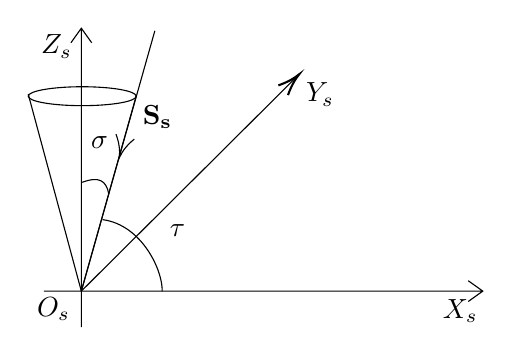
\begin{tikzpicture}[x=0.75pt,y=0.75pt,yscale=-1,xscale=1]
%uncomment if require: \path (0,300); %set diagram left start at 0, and has height of 300

%Shape: Axis 2D [id:dp15254390994019373] 
\draw  (191,193.66) -- (402.5,193.66)(209.08,67) -- (209.08,211) (395.5,188.66) -- (402.5,193.66) -- (395.5,198.66) (204.08,74) -- (209.08,67) -- (214.08,74)  ;
%Straight Lines [id:da015010332337416443] 
\draw    (209.08,193.66) -- (312.66,90.57) ;
\draw [shift={(314.08,89.16)}, rotate = 135.14] [color={rgb, 255:red, 0; green, 0; blue, 0 }  ][line width=0.75]    (10.93,-3.29) .. controls (6.95,-1.4) and (3.31,-0.3) .. (0,0) .. controls (3.31,0.3) and (6.95,1.4) .. (10.93,3.29)   ;
%Straight Lines [id:da4823254861761963] 
\draw    (183.5,98.75) -- (209.08,193.66) ;
%Straight Lines [id:da5054606356463616] 
\draw    (209.08,193.66) -- (235.5,99.75) ;
%Shape: Ellipse [id:dp4424595462059493] 
\draw   (183.5,99.75) .. controls (183.5,97.23) and (195.14,95.19) .. (209.5,95.19) .. controls (223.86,95.19) and (235.5,97.23) .. (235.5,99.75) .. controls (235.5,102.27) and (223.86,104.31) .. (209.5,104.31) .. controls (195.14,104.31) and (183.5,102.27) .. (183.5,99.75) -- cycle ;
\draw   (234.58,120.45) .. controls (231.2,123.17) and (228.8,126.17) .. (227.37,129.44) .. controls (227.82,125.9) and (227.28,122.09) .. (225.78,118.02) ;
%Straight Lines [id:da27770596173012896] 
\draw    (209.08,193.66) -- (244.5,68.25) ;
%Curve Lines [id:da9717802058822778] 
\draw    (209.5,141.25) .. controls (217.5,138.25) and (221,140.25) .. (222.29,146.71) ;
%Curve Lines [id:da7681816573118487] 
\draw    (219.29,159.21) .. controls (238.5,161.75) and (248.5,184.25) .. (248,193.75) ;

% Text Node
\draw (316.08,92.16) node [anchor=north west][inner sep=0.75pt]   [align=left] {$\displaystyle Y_{s}$};
% Text Node
\draw (382,196.5) node [anchor=north west][inner sep=0.75pt]   [align=left] {$\displaystyle X_{s}$};
% Text Node
\draw (188.5,69) node [anchor=north west][inner sep=0.75pt]   [align=left] {$\displaystyle Z_{s}$};
% Text Node
\draw (186.5,195.5) node [anchor=north west][inner sep=0.75pt]   [align=left] {$\displaystyle O_{s}$};
% Text Node
\draw (237.5,102.75) node [anchor=north west][inner sep=0.75pt]   [align=left] {$\displaystyle \mathbf{S_{s}}$};
% Text Node
\draw (212.5,118) node [anchor=north west][inner sep=0.75pt]   [align=left] {$\displaystyle \sigma $};
% Text Node
\draw (250.5,160.5) node [anchor=north west][inner sep=0.75pt]   [align=left] {$\displaystyle \tau $};


\end{tikzpicture}

\end{center}\caption{太阳光锥坐标系示意图}\label{gz}
\end{figure}

假设这一束光锥中光线$S_s$与来自太阳中心的主光线的夹角为$\sigma$,与$X_s$轴夹角为$\tau$,则该光线的方向向量为:

\begin{eqnarray}
\mathbf{S_s}=(\sin \sigma\cos \tau,\sin\sigma\sin\tau,\cos\sigma)
\end{eqnarray}

\subsection{截断效率的计算}
从坐标系$H_s$下转换到镜场坐标系$H_0$的旋转矩阵为$\mathbf{T_S}$,以该光锥中光线$S_s$为例,计算该光线经反射后到达吸热器上的落点坐标,计算步骤如下:
\begin{enumerate}[label=$Step$ \arabic*:, leftmargin=*]
\item 将坐标$H_1|_{H_A}$转换到坐标系$H_0$下:
\begin{eqnarray}
H_1(x_1',y_1',z_1')|_{H_0}=\mathbf{T_A}\cdot H_1|_{H_A}
\end{eqnarray}
\item 将该光线由太阳光锥坐标系$H_s$转换到镜场坐标系$H_0$:
\begin{eqnarray}
\mathbf{S_s}|_{H_0}=\mathbf{T_S}\cdot \mathbf{S_s}|_{H_s}
\end{eqnarray}
\item 将坐标系$H_A$法向量转换到坐标系$H_0$下坐标:
\begin{eqnarray}
\mathbf{OZ_A}|_{H_0}=\mathbf{T_A}\cdot \mathbf{OZ_A}|_{H_A}
\end{eqnarray}
\item 计算反射向量$\mathbf{S_s'}=(m,n,l)$:
\begin{eqnarray}
\frac{\mathbf{S_s}|_{H_0}-\mathbf{S_s'}|_{H_0}}{2}=-\mathbf{OZ_A}|_{H_0}
\end{eqnarray}
\item 计算该光线经镜面反射后射向吸收塔的方程:
\begin{eqnarray}
\frac{x-x'_1}{m}=\frac{y-y_1'}{n}=\frac{z-z_1'}{l}
\end{eqnarray}
\item 计算集热器方程$J$:
\begin{eqnarray}
J=\left\{\begin{matrix}
x^2+y^2=\frac{49}{4} \\
z\in[76,84]
\end{matrix}\right.
\end{eqnarray}
\item 设计算法判断该光线是否落入集热器中.
\end{enumerate}

我们的算法思路是判断当$z$值由集热器底部变化到集热器顶部时,观测$x^2+y^2$的值是否落入集热器范围内。即通过观测二次函数$G(z-4)$观测值的变化,来判断光线是否落入集热器范围内。其中观测函数如下:
\begin{eqnarray}
G(z-4)=x^2+y^2=x_1'^2+y_1'^2+\frac{1}{l^2}(m^2+n^2)(z-4)^2+\frac{2}{l}(ny_1'+mx_1')(z-4)
\end{eqnarray}

我们使用蒙特卡洛光际追踪方法计算各定日镜的截断效率,算法伪代码如下:

\begin{algorithm}[H]
\normalem
  \SetAlgoLined
  \KwIn{定日镜坐标及其法向量}
 
  \KwOut{截断效率$\eta_{trunc}$}
  
  \For{定日镜}
  {$X=0$ \;
  \textbf{rand}\ $X_1$个坐标$H|_{H_A}$ \;
  \textbf{rand}\ $X_2$个$\sigma,\tau$ \;
   \For{H}
   {
    $H_1|_{H_A}\longmapsto H_1|_{H_0}$ \;
    $\mathbf{S_s}|_{H_s}\longmapsto \mathbf{S_s}|_{H_0}$ \;
    $\mathbf{OZ_A}|_{H_A}\longmapsto \mathbf{OZ_A}|_{H_0}$ \;
    \textbf{calculate} $\mathbf{S_s'}|_{H_0}$ \;
    $X=X+\textbf{find(}(x,y,z)s.t.G(z-4)\le r^2\textbf{)}$ \;
   }
   \textbf{calculate}\ $\eta_{trunc}=\frac{X}{X_1X_2}$ \;
  }  
  \caption{蒙特卡洛光际追踪算法计算截断效率}
 \end{algorithm}
\subsection{问题一求解及结果展示}
根据题目所给条件,对于定日镜$i$,其光学效率计算如下:
\begin{eqnarray}
\eta_i=\eta_{sb}\eta_{cos}\eta_{at}\eta_{trunc}\eta_{ref}
\end{eqnarray}
在实际计算时,我们取镜面反射率$\eta_{ref}=0.92$为常数。

定日镜场的输出热功率$E_{field}$计算如下:
\begin{eqnarray}
E_{field}=\text{DNI}\cdot \sum_i^NA_i\eta_i
\end{eqnarray}
单位镜面面积输出热功率$\hat{E}$计算如下:
\begin{eqnarray}
\hat{E}=\frac{\hat{E}_{filed}}{\sum\limits_i^N\eta_i}
\end{eqnarray}

为了更加直观看到镜场的效率分布,我们将各季度定日镜场的平均光学效率分布云图展示在图\ref{a3}中,并根据题目计算得到该定日镜场的年平均光学效率、年平均输出热功率,以及单位镜面面积年平均输出热功率,结果见表\ref{a1}和表\ref{a2}:

\begin{figure}[H]
\centering
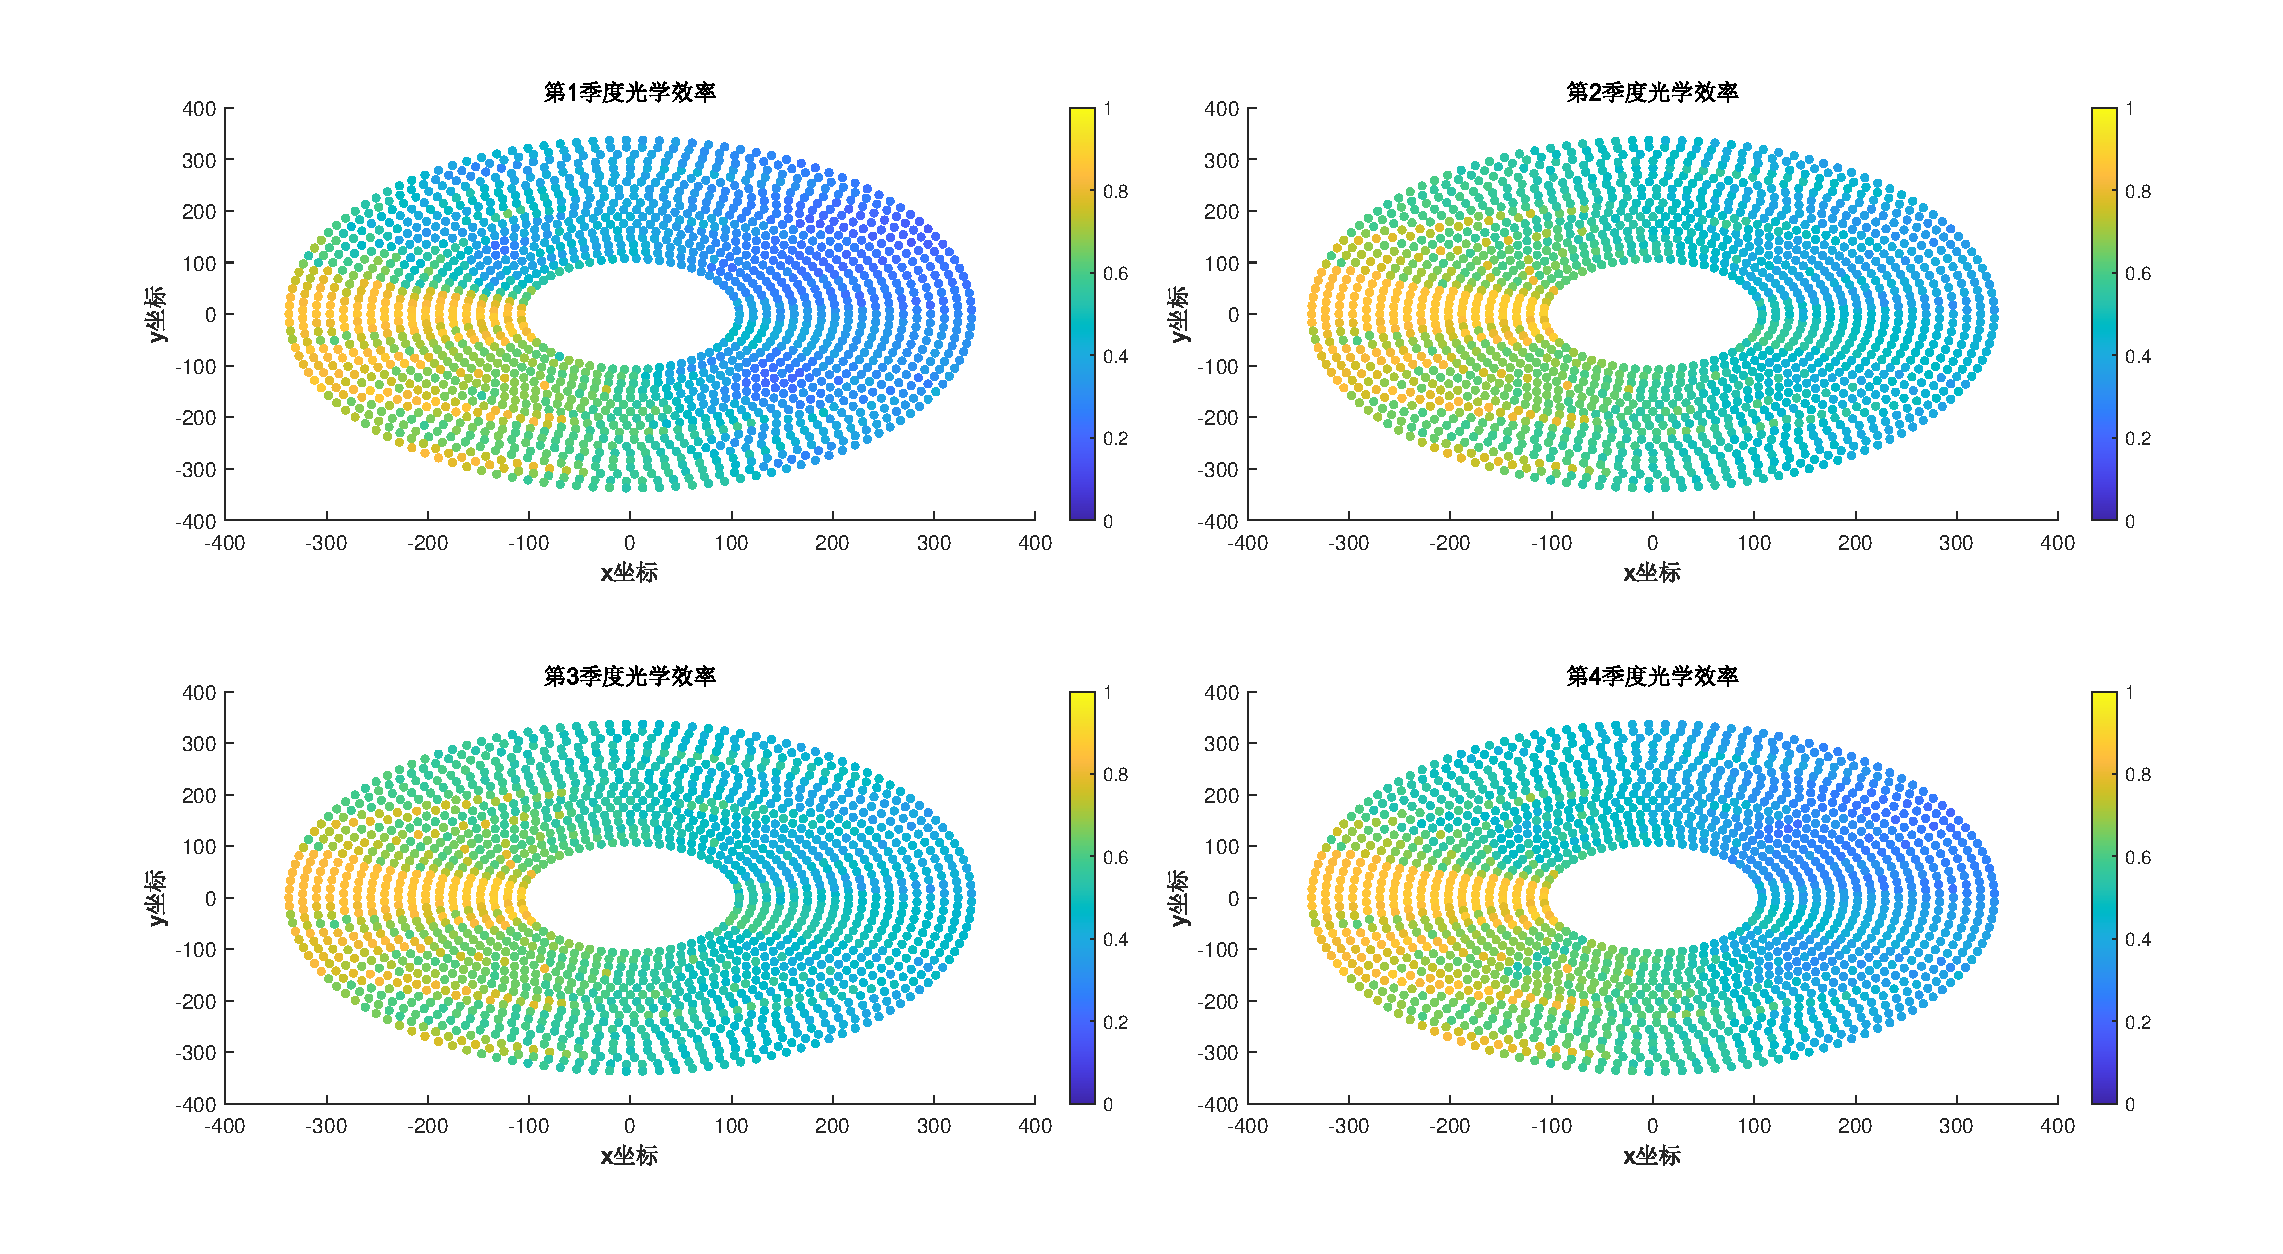
\includegraphics[height=.56\textwidth]{figures/热力图.eps}
\caption{各季度镜场光学效率分布云图}\label{a3}
\end{figure}


\begin{table}[H]
\centering
\caption{问题一每月 21 日平均光学效率及输出功率}
\label{a1}\resizebox{\textwidth}{!}{
\begin{tabular}{@{}cccccc@{}}
\toprule
日期     & 平均光学效率      & 平均余弦效率   & 平均阴影遮挡效率 & 平均截断效率      & 单位面积镜面平均输出热功率 ($kW/m^2$) \\ \midrule
1月21日  & 0.510092357 & 0.722664 & 0.969717 & 0.749377247 & 0.44316821                 \\
2月21日  & 0.541176829 & 0.743589 & 0.999520 & 0.791058057 & 0.50962610                   \\
3月21日  & 0.556968774 & 0.764687 & 0.999956 & 0.794804739 & 0.55362690                  \\
4月21日  & 0.570695666 & 0.783219 & 1.000000       & 0.806004132 & 0.58701754
                    \\
5月21日  & 0.578219692 & 0.793373 & 1.000000 & 0.842930100   & 0.60389261
                    \\
6月21日  & 0.580518545 & 0.796468 & 1.000000        & 0.998000000       & 0.60884781
                   \\
7月21日  & 0.578140295 & 0.793266 & 1.000000        & 0.985000000       & 0.60369409
                  \\
8月21日  & 0.570162593 & 0.782504 & 0.999994 & 0.791058057 & 0.58578503
                  \\
9月21日  & 0.556184734 & 0.763619 & 0.999965 & 0.785403253 & 0.55156837
                  \\
10月21日 & 0.533494724 & 0.740932 & 0.988660  & 0.783848306 & 0.49823073
                   \\
11月21日 & 0.496591115 & 0.720886 & 0.946943 & 0.777444109 & 0.42771388
                   \\
12月21日 & 0.488376666 & 0.713619 & 0.941274 & 0.763523659 & 0.40422933
                   \\ \bottomrule
\end{tabular}}
\end{table}
\begin{table}[H]
\centering
\caption{问题一年平均光学效率及输出功率表}
\label{a2}\resizebox{\textwidth}{!}{
\begin{tabular}{@{}cccccc@{}}
\toprule
年平均光学效率 &
年平均余弦效率 &
  年平均阴影遮挡效率 &
年平均截断效率 &
  年平均输出热功率 ($MW$) &
  单位面积镜面年平均输出热功率 ($kW/m^2$) \\ \midrule
0.546718499 &
  0.759902 &
  0.987169083 &
  0.82211874 &
  33.382548 &
  0.5314 \\ \bottomrule
\end{tabular}}
\end{table}
\section{第二问模型建立与求解}
针对问题二,题目要求我们在满足定日镜场的额定年平均输入热功率为60MW,对定日镜的尺寸和安装高度等进行合理的优化安排使得单位镜面面积年平均输出热功率尽量大。在问题一的求解过程中,发现了基本布局存在着疏密放置等方面的问题,所以接下来我们依据题目要求对定日镜场的布局进行优化:
\subsection{布局优化}
DELSOL3型布局考虑规则的径向交错定日镜场(见图\ref{del}),该方式能有效的降低阴影/遮挡效率损失,提高土地利用率和大气衰减效率。$^\text{\cite{xxxxxxxx}}$$^\text{\cite{xxxxxxxxx}}$$^\text{\cite{xxxxxxxxxx}}$
\begin{figure}[H]
\begin{center}

\tikzset{every picture/.style={line width=0.75pt}} %set default line width to 0.75pt        

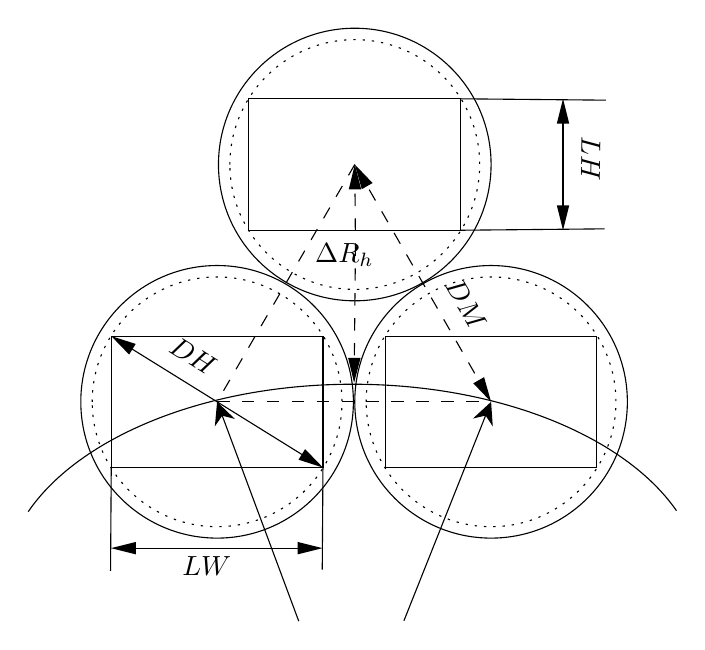
\begin{tikzpicture}[x=0.75pt,y=0.75pt,yscale=-1,xscale=1]
%uncomment if require: \path (0,300); %set diagram left start at 0, and has height of 300

%Shape: Circle [id:dp004225071928420254] 
\draw   (131.33,60.33) .. controls (131.33,24.07) and (160.73,-5.33) .. (197,-5.33) .. controls (233.27,-5.33) and (262.67,24.07) .. (262.67,60.33) .. controls (262.67,96.6) and (233.27,126) .. (197,126) .. controls (160.73,126) and (131.33,96.6) .. (131.33,60.33) -- cycle ;
%Shape: Circle [id:dp12314767814749206] 
\draw   (65,174.67) .. controls (65,138.4) and (94.4,109) .. (130.67,109) .. controls (166.93,109) and (196.33,138.4) .. (196.33,174.67) .. controls (196.33,210.93) and (166.93,240.33) .. (130.67,240.33) .. controls (94.4,240.33) and (65,210.93) .. (65,174.67) -- cycle ;
%Shape: Circle [id:dp22460770681959596] 
\draw   (197,174.67) .. controls (197,138.4) and (226.4,109) .. (262.67,109) .. controls (298.93,109) and (328.33,138.4) .. (328.33,174.67) .. controls (328.33,210.93) and (298.93,240.33) .. (262.67,240.33) .. controls (226.4,240.33) and (197,210.93) .. (197,174.67) -- cycle ;
%Shape: Circle [id:dp8064458051993861] 
\draw  [dash pattern={on 0.84pt off 2.51pt}] (136.83,60.33) .. controls (136.83,27.1) and (163.77,0.17) .. (197,0.17) .. controls (230.23,0.17) and (257.17,27.1) .. (257.17,60.33) .. controls (257.17,93.56) and (230.23,120.5) .. (197,120.5) .. controls (163.77,120.5) and (136.83,93.56) .. (136.83,60.33) -- cycle ;
%Shape: Circle [id:dp9011822713711417] 
\draw  [dash pattern={on 0.84pt off 2.51pt}] (70.5,174.67) .. controls (70.5,141.44) and (97.44,114.5) .. (130.67,114.5) .. controls (163.9,114.5) and (190.83,141.44) .. (190.83,174.67) .. controls (190.83,207.9) and (163.9,234.83) .. (130.67,234.83) .. controls (97.44,234.83) and (70.5,207.9) .. (70.5,174.67) -- cycle ;
%Shape: Circle [id:dp4795358037927018] 
\draw  [dash pattern={on 0.84pt off 2.51pt}] (202.5,174.67) .. controls (202.5,141.44) and (229.44,114.5) .. (262.67,114.5) .. controls (295.9,114.5) and (322.83,141.44) .. (322.83,174.67) .. controls (322.83,207.9) and (295.9,234.83) .. (262.67,234.83) .. controls (229.44,234.83) and (202.5,207.9) .. (202.5,174.67) -- cycle ;
%Shape: Rectangle [id:dp6535781553197324] 
\draw   (146,28.67) -- (248,28.67) -- (248,92) -- (146,92) -- cycle ;
%Shape: Rectangle [id:dp9962018095206184] 
\draw   (79.67,143) -- (181.67,143) -- (181.67,206.33) -- (79.67,206.33) -- cycle ;
%Shape: Rectangle [id:dp9347627422342439] 
\draw   (211.67,143) -- (313.67,143) -- (313.67,206.33) -- (211.67,206.33) -- cycle ;
%Straight Lines [id:da6959667056738195] 
\draw  [dash pattern={on 4.5pt off 4.5pt}]  (198,62.07) -- (261.67,172.93) ;
\draw [shift={(262.67,174.67)}, rotate = 240.13] [fill={rgb, 255:red, 0; green, 0; blue, 0 }  ][line width=0.08]  [draw opacity=0] (12,-3) -- (0,0) -- (12,3) -- cycle    ;
\draw [shift={(197,60.33)}, rotate = 60.13] [fill={rgb, 255:red, 0; green, 0; blue, 0 }  ][line width=0.08]  [draw opacity=0] (12,-3) -- (0,0) -- (12,3) -- cycle    ;
%Straight Lines [id:da03392881691633143] 
\draw    (248,28.67) -- (318,29.33) ;
%Straight Lines [id:da7802632435961052] 
\draw    (248,92) -- (317.33,91.33) ;
%Straight Lines [id:da6755325225657745] 
\draw    (297.33,30.67) -- (297.33,90) ;
\draw [shift={(297.33,92)}, rotate = 270] [fill={rgb, 255:red, 0; green, 0; blue, 0 }  ][line width=0.08]  [draw opacity=0] (12,-3) -- (0,0) -- (12,3) -- cycle    ;
\draw [shift={(297.33,28.67)}, rotate = 90] [fill={rgb, 255:red, 0; green, 0; blue, 0 }  ][line width=0.08]  [draw opacity=0] (12,-3) -- (0,0) -- (12,3) -- cycle    ;
%Shape: Arc [id:dp4879452297069622] 
\draw  [draw opacity=0] (39.67,227.59) .. controls (64.23,191.65) and (124.94,166.21) .. (195.96,166.19) .. controls (266.71,166.18) and (327.25,191.42) .. (352,227.14) -- (195.98,263.11) -- cycle ; \draw   (39.67,227.59) .. controls (64.23,191.65) and (124.94,166.21) .. (195.96,166.19) .. controls (266.71,166.18) and (327.25,191.42) .. (352,227.14) ;  
%Straight Lines [id:da1576505248863267] 
\draw  [dash pattern={on 4.5pt off 4.5pt}]  (197.02,62.33) -- (197.33,100.17) -- (196.69,163.5) ;
\draw [shift={(196.67,165.5)}, rotate = 270.58] [fill={rgb, 255:red, 0; green, 0; blue, 0 }  ][line width=0.08]  [draw opacity=0] (12,-3) -- (0,0) -- (12,3) -- cycle    ;
\draw [shift={(197,60.33)}, rotate = 89.52] [fill={rgb, 255:red, 0; green, 0; blue, 0 }  ][line width=0.08]  [draw opacity=0] (12,-3) -- (0,0) -- (12,3) -- cycle    ;
%Straight Lines [id:da37986651980220176] 
\draw  [dash pattern={on 4.5pt off 4.5pt}]  (197,60.33) -- (130.67,174.67) ;
%Straight Lines [id:da07922120024906842] 
\draw  [dash pattern={on 4.5pt off 4.5pt}]  (130.67,174.67) -- (262.67,174.67) ;
%Straight Lines [id:da2671795512962303] 
\draw    (81.37,144.06) -- (130.67,174.67) -- (179.97,205.28) ;
\draw [shift={(181.67,206.33)}, rotate = 211.84] [fill={rgb, 255:red, 0; green, 0; blue, 0 }  ][line width=0.08]  [draw opacity=0] (12,-3) -- (0,0) -- (12,3) -- cycle    ;
\draw [shift={(79.67,143)}, rotate = 31.84] [fill={rgb, 255:red, 0; green, 0; blue, 0 }  ][line width=0.08]  [draw opacity=0] (12,-3) -- (0,0) -- (12,3) -- cycle    ;
%Straight Lines [id:da283237583343354] 
\draw    (79.33,256.17) -- (79.67,206.33) ;
%Straight Lines [id:da767522769428975] 
\draw    (181.33,255.5) -- (181.67,206.33) ;
%Straight Lines [id:da28042671125268037] 
\draw    (81.5,245.17) -- (179.5,245.17) ;
\draw [shift={(181.5,245.17)}, rotate = 180] [fill={rgb, 255:red, 0; green, 0; blue, 0 }  ][line width=0.08]  [draw opacity=0] (12,-3) -- (0,0) -- (12,3) -- cycle    ;
\draw [shift={(79.5,245.17)}, rotate = 0] [fill={rgb, 255:red, 0; green, 0; blue, 0 }  ][line width=0.08]  [draw opacity=0] (12,-3) -- (0,0) -- (12,3) -- cycle    ;
%Straight Lines [id:da27880648165827937] 
\draw    (170,280.33) -- (131.71,177.48) ;
\draw [shift={(130.67,174.67)}, rotate = 69.58] [fill={rgb, 255:red, 0; green, 0; blue, 0 }  ][line width=0.08]  [draw opacity=0] (10.72,-5.15) -- (0,0) -- (10.72,5.15) -- (7.12,0) -- cycle    ;
%Straight Lines [id:da5960639528771248] 
\draw    (220.67,280.17) -- (261.56,177.45) ;
\draw [shift={(262.67,174.67)}, rotate = 111.71] [fill={rgb, 255:red, 0; green, 0; blue, 0 }  ][line width=0.08]  [draw opacity=0] (10.72,-5.15) -- (0,0) -- (10.72,5.15) -- (7.12,0) -- cycle    ;

% Text Node
\draw (248.7,112.43) node [anchor=north west][inner sep=0.75pt]  [rotate=-60.02] [align=left] {$\displaystyle DM$};
% Text Node
\draw (316.7,45.98) node [anchor=north west][inner sep=0.75pt]  [rotate=-90.97] [align=left] {$\displaystyle LH$};
% Text Node
\draw (176.67,97.33) node [anchor=north west][inner sep=0.75pt]   [align=left] {$\displaystyle \Delta R_{h}$};
% Text Node
\draw (111.27,140.78) node [anchor=north west][inner sep=0.75pt]  [rotate=-32.19] [align=left] {$\displaystyle DH$};
% Text Node
\draw (112.67,248) node [anchor=north west][inner sep=0.75pt]   [align=left] {$\displaystyle LW$};


\end{tikzpicture}
\caption{DELSOL3型分布示意图}\label{del}
\end{center}
\end{figure}

考虑定日镜宽为$LH$,定日镜高为$LW$,安装高度为$RH$,则有:
\begin{eqnarray}
LH\le RH\le 6
\end{eqnarray}
\begin{eqnarray}
2\le LW\le LH\le 8
\end{eqnarray}

定义$DM$表示为镜面中心间距离,$DH$表示为定日镜镜面对角线长度,考虑定日镜间不能发生机械碰撞且相邻镜面中心间距离比镜面宽度多$5m$以上,则有:

\begin{eqnarray}
DH=\sqrt{LH^2+LW^2}
\end{eqnarray}
\begin{eqnarray}
DM\ge LH+5
\end{eqnarray}

我们给定吸收塔位置为镜场坐标系原点,即点$(0,0)$,第一行首个的定日镜中心坐标我们给出为$(100+\frac{DH}{2},0)$,定义基本环为该环$y$轴方向存在定日镜,交错环为该环$y$轴方向不存在定日镜,以一个基本环加上交错环作为一个基本区域,我们首先计算得到第一个行定日镜数目为$N$,则第一个基本区域的定日镜数量为$2N$,由几何知识可知下一区域内各行的定日镜数量为上一个基本区域的定日镜数量的两倍,即该区域内定日镜数量为$4N$,假设我们有$n$个基本区域,则初始总定日镜数量为$(2^{n+1}-1)\cdot N$。由题目要求可以得到布置区域距吸收塔范围在$[R_{\min},R_{\max}]$之间定义相邻行之间的最小增量为$\Delta R_h$,相邻区域之间最小增量为$\Delta R_f$,则有:

\begin{eqnarray}
\Delta R_h=\frac{\sqrt{3}DM}{2}-R_1+\sqrt{R_1+\frac{DM^2}{4}}
\end{eqnarray}
\begin{eqnarray}
\Delta R_f=DM
\end{eqnarray}
\subsection{问题二求解及结果展示}
对于大规模优化问题,我们可以列出目标函数列出约束条件利用优化算法求解,但是在本文中,可以使用SolarPILOT(Solar Power Tower Integrated Layout and OptimizationTool)软件进行仿真模拟,在镜场参数给定的情况下,收敛速率和求解精度均能够得到保证。$^\text{\cite{z}}$

SolarPILOT的主要功能包括模拟和优化各种类型的太阳能热发电技术,如塔式太阳能热电联产系统、槽式太阳能热电联产系统和抛物面太阳能反射器系统等。使用COBYLA算法(NLOpt库的一部分)来优化所选变量。该算法将目标函数表示为局部信任区域内的多维线性曲面,并使用约束边界的线性近似来合并非线性约束。可以考虑到太阳能的光照强度、太阳位置、镜面和反射器的特性以及其他因素,通过数值计算来预测系统的性能。$^\text{\cite{xxxxxxxxxxx}}$$^\text{\cite{xxxxxxxxxxxx}}$$^\text{\cite{xxxxxxxxxxxxx}}$

接下来我们使用 SolarPILOT 软件平台进行仿真模拟,布局优化后我们将初始数值在Field Layout界面进行导入并运行。给出流程图见图\ref{lct}:
\begin{figure}[H]
\centering
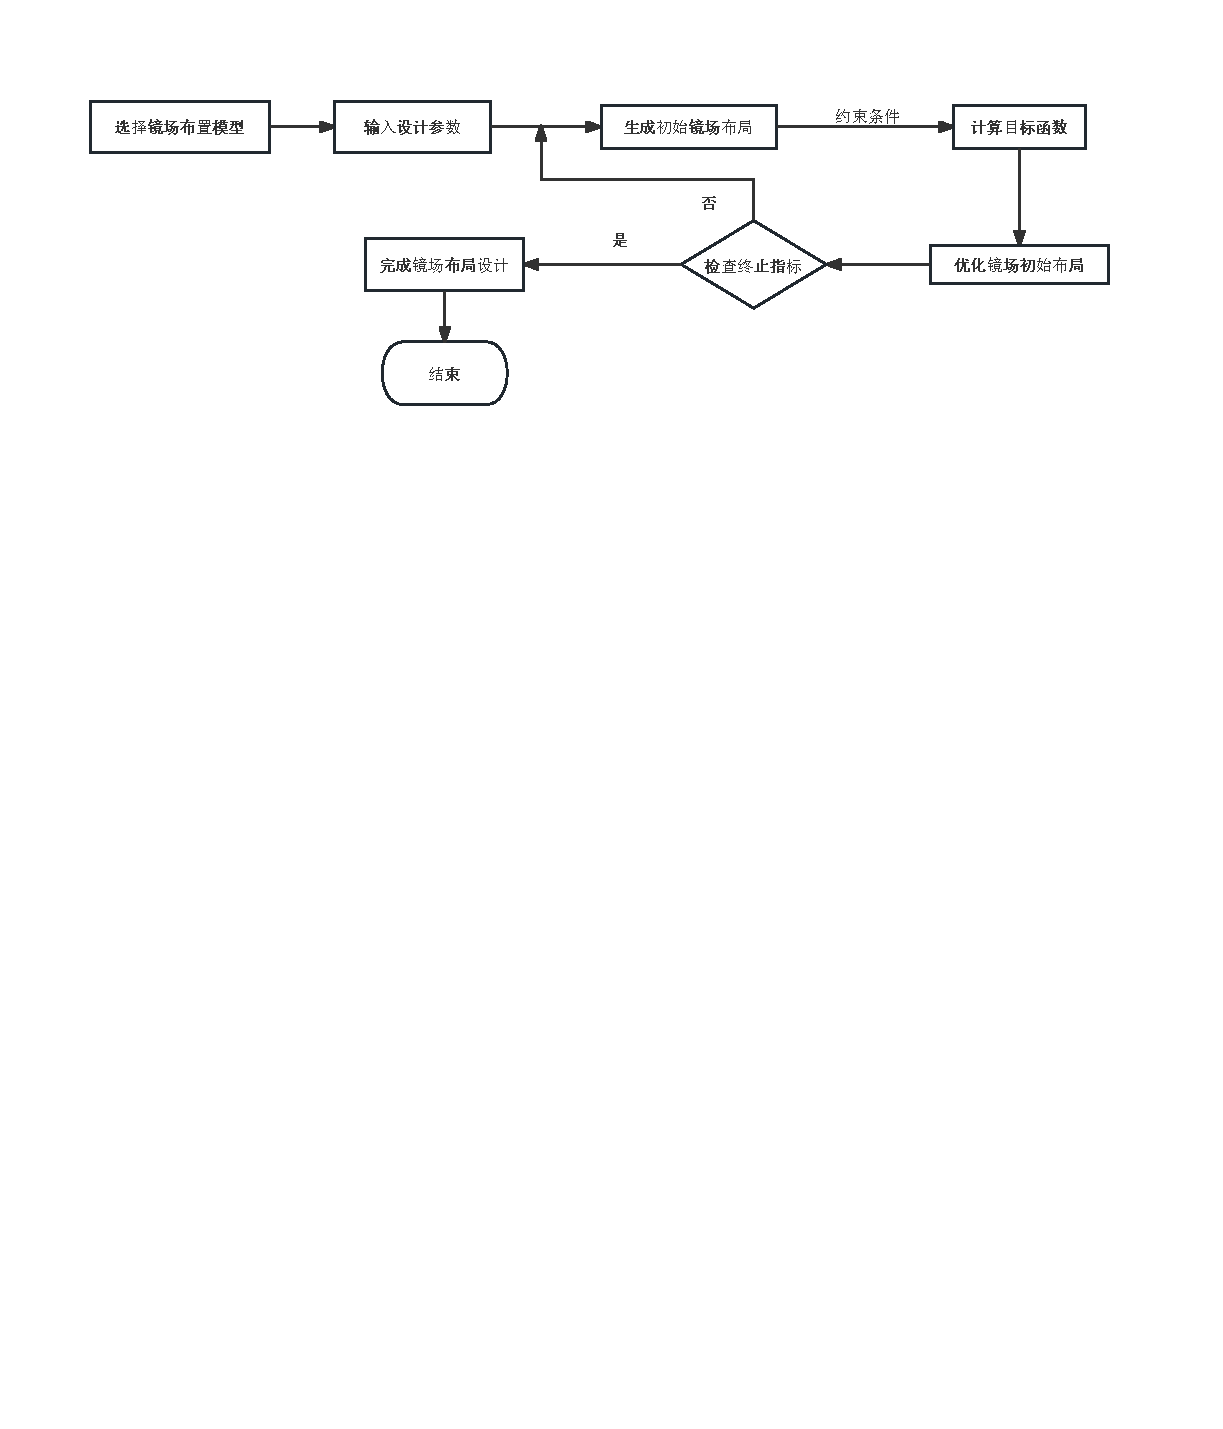
\includegraphics[width=\textwidth]{figures/未命名文件.pdf}
\caption{求解流程图}\label{lct}
\end{figure}

软件具体操作步骤如下:
\begin{enumerate}[label=$Step$ \arabic*:, leftmargin=*]
\item 在Climate界面选择China CHN Mangnai(INTL).csv,也就是经纬度及海拔最接近题目所给背景的地点作为定日镜场地的模拟地点。
\item 在Layout Setup界面对定日镜场的设计功率、吸收塔光学高度及场地范围进行约束。
\item 在Receiver 1界面设置集热器的高度和直径,到此即完成了初始模型的建立。
\item 在Parametrics界面点击Add选择”Structure height”和”Structure width”,也就是定日镜长度、宽度及高度进行约束及优化,长度和宽度的优化范围为[2,8],高度的优化范围为[2,6],步长定为0.1,运行。
\item 将运行所得结果导出为csv格式,并对文件中数据进行筛选处理,选择单位镜面面积年平均输出热功率最大的一组数据。
\item 将所得最优长度宽度及高度在Template 1界面进行输入并运行,然后在Parametrics界面选择相关方位间距因子进行约束优化,优化范围设置为[12.3,20],步长定为0.1,进行优化。
\item 同$Step \  5$,筛选处理并选取定日镜底座中心间距的最优数据。
\item 在Optimization界面选择“Tower location offset-X”“Tower location offset-Y”,对中心吸收塔的位置进行约束优化,优化范围为[-350,350],步长定为0.01,进行多次优化调整,最终得出塔的最优位置。
\item 在Filed Layout界面对优化后的模型进行运行,得出结论图像,保存相关图像,详细结果见图\ref{cxqd}:
\begin{figure}[htbp]
\centering
\begin{subfigure}[b]{.49\textwidth}
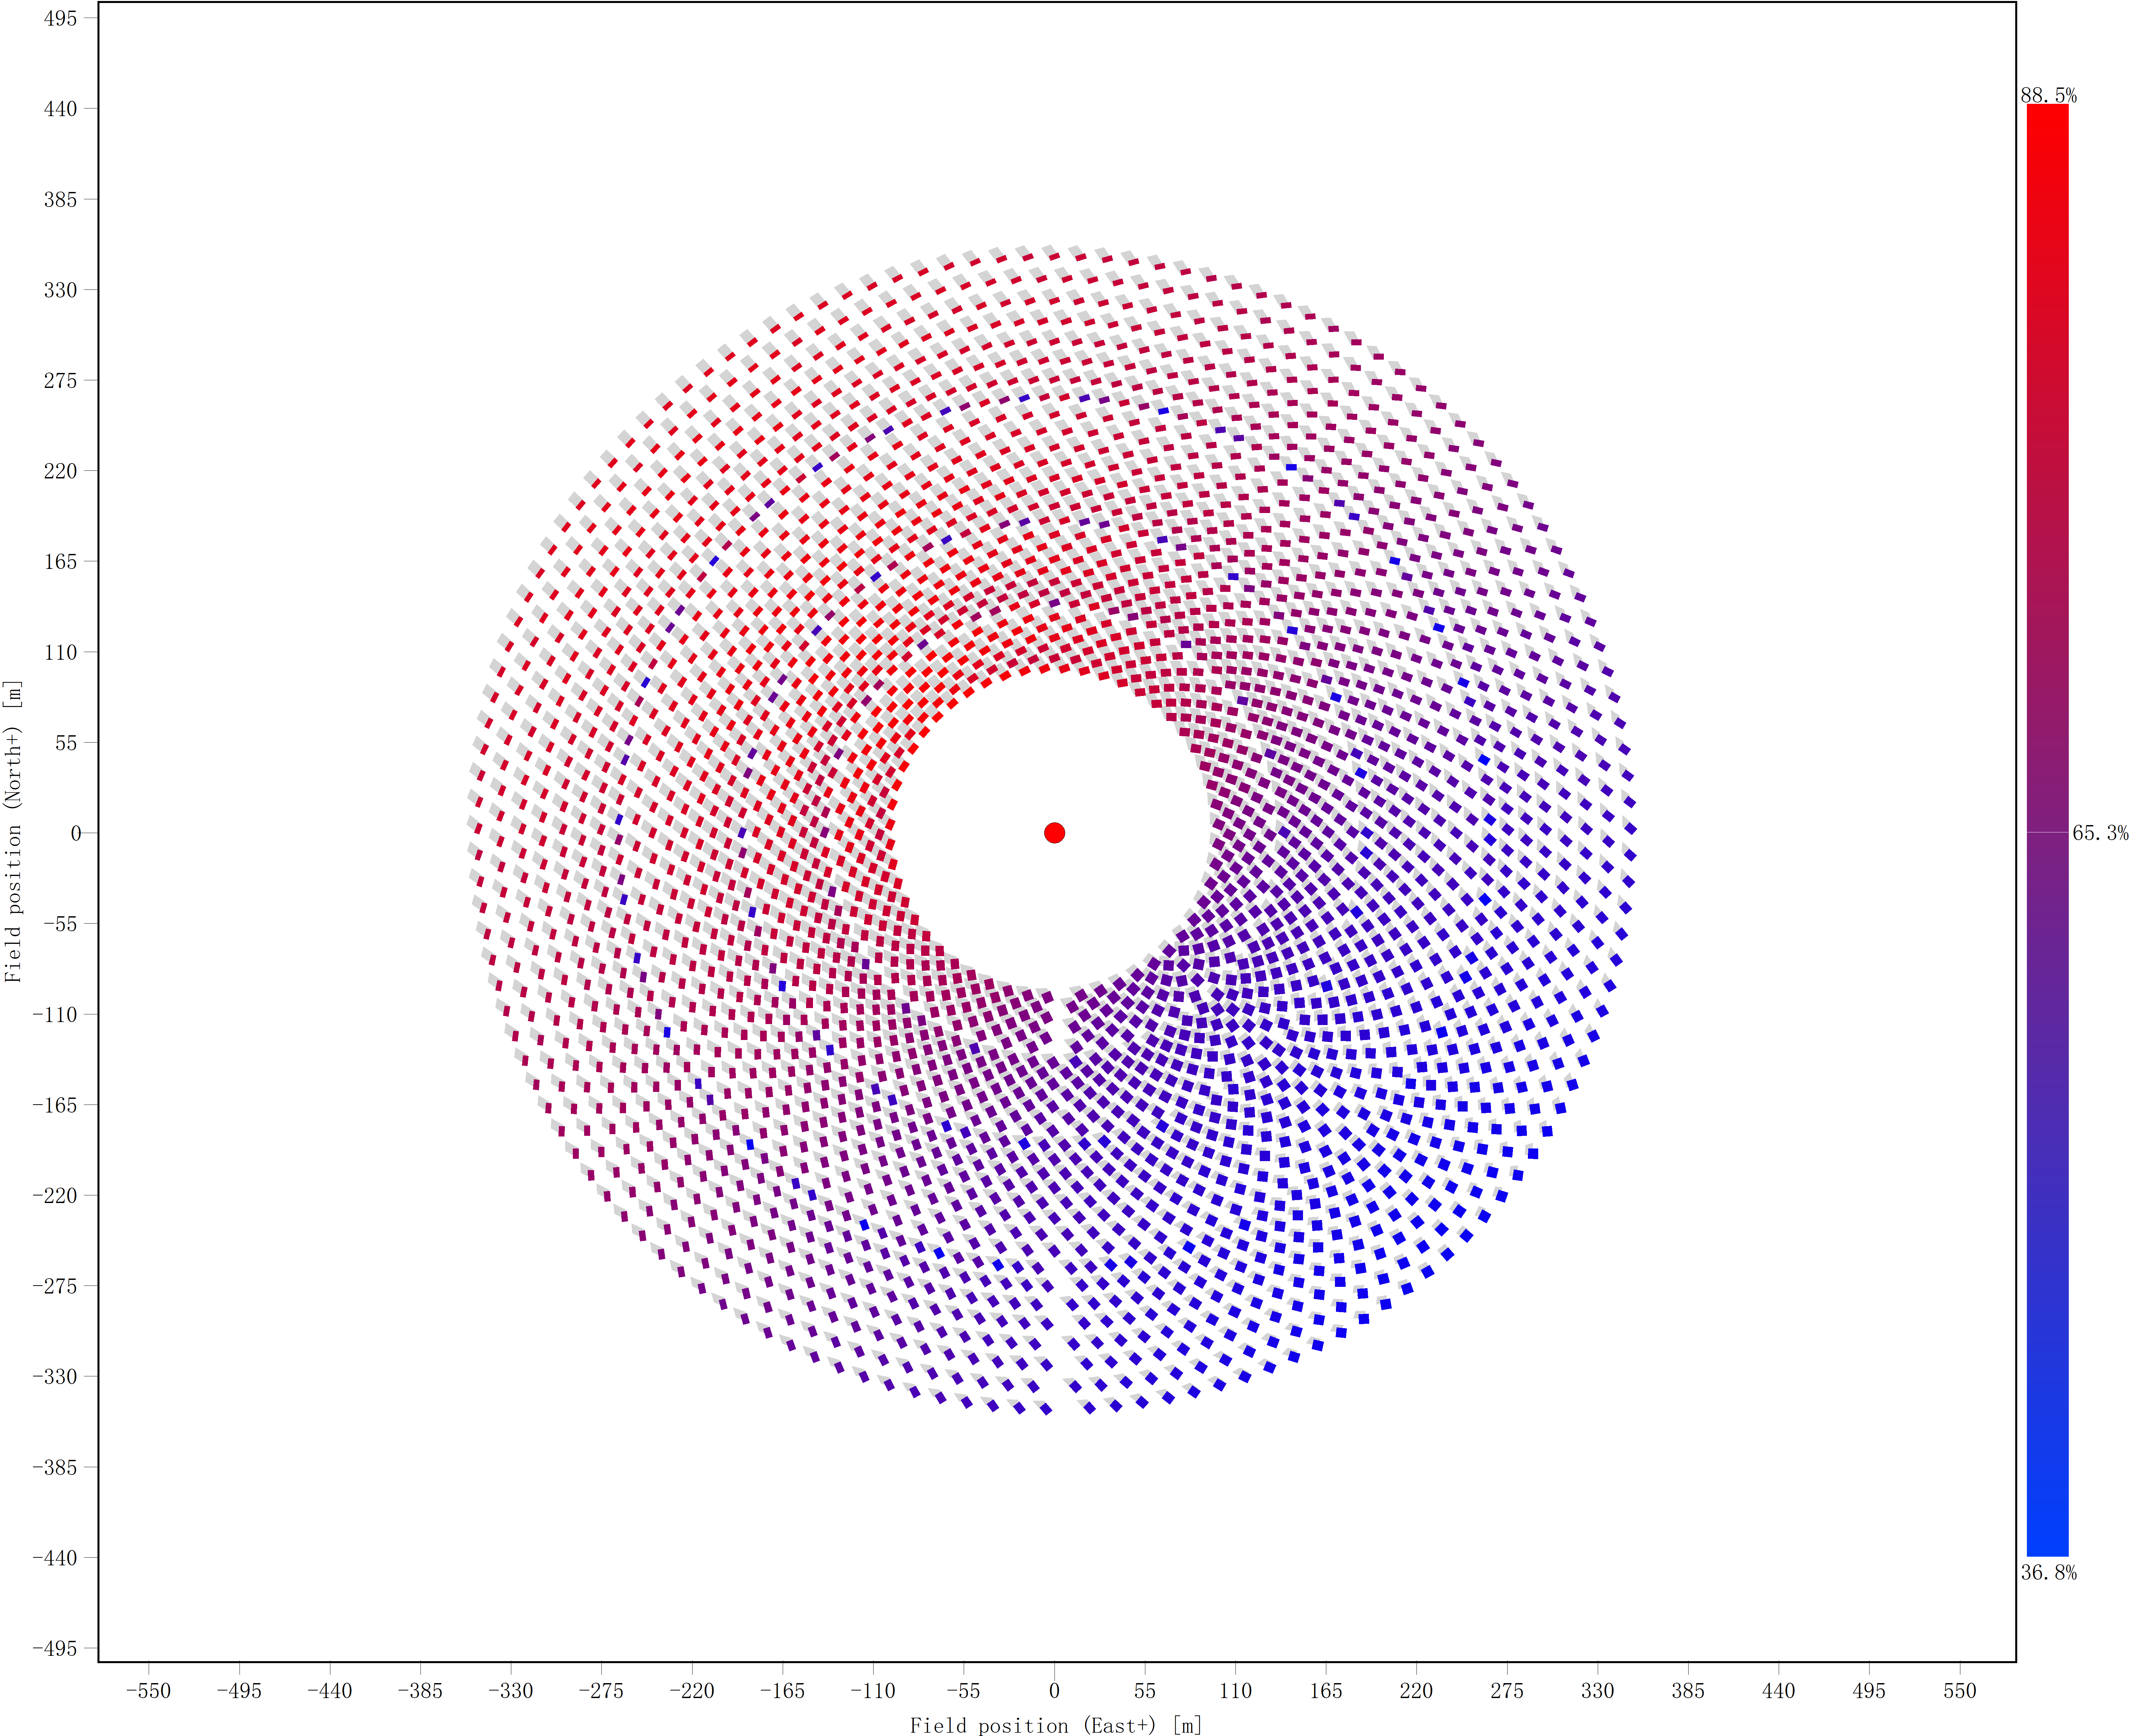
\includegraphics[width=\textwidth]{figures/2682春分.png}
\end{subfigure}
\begin{subfigure}[b]{.49\textwidth}
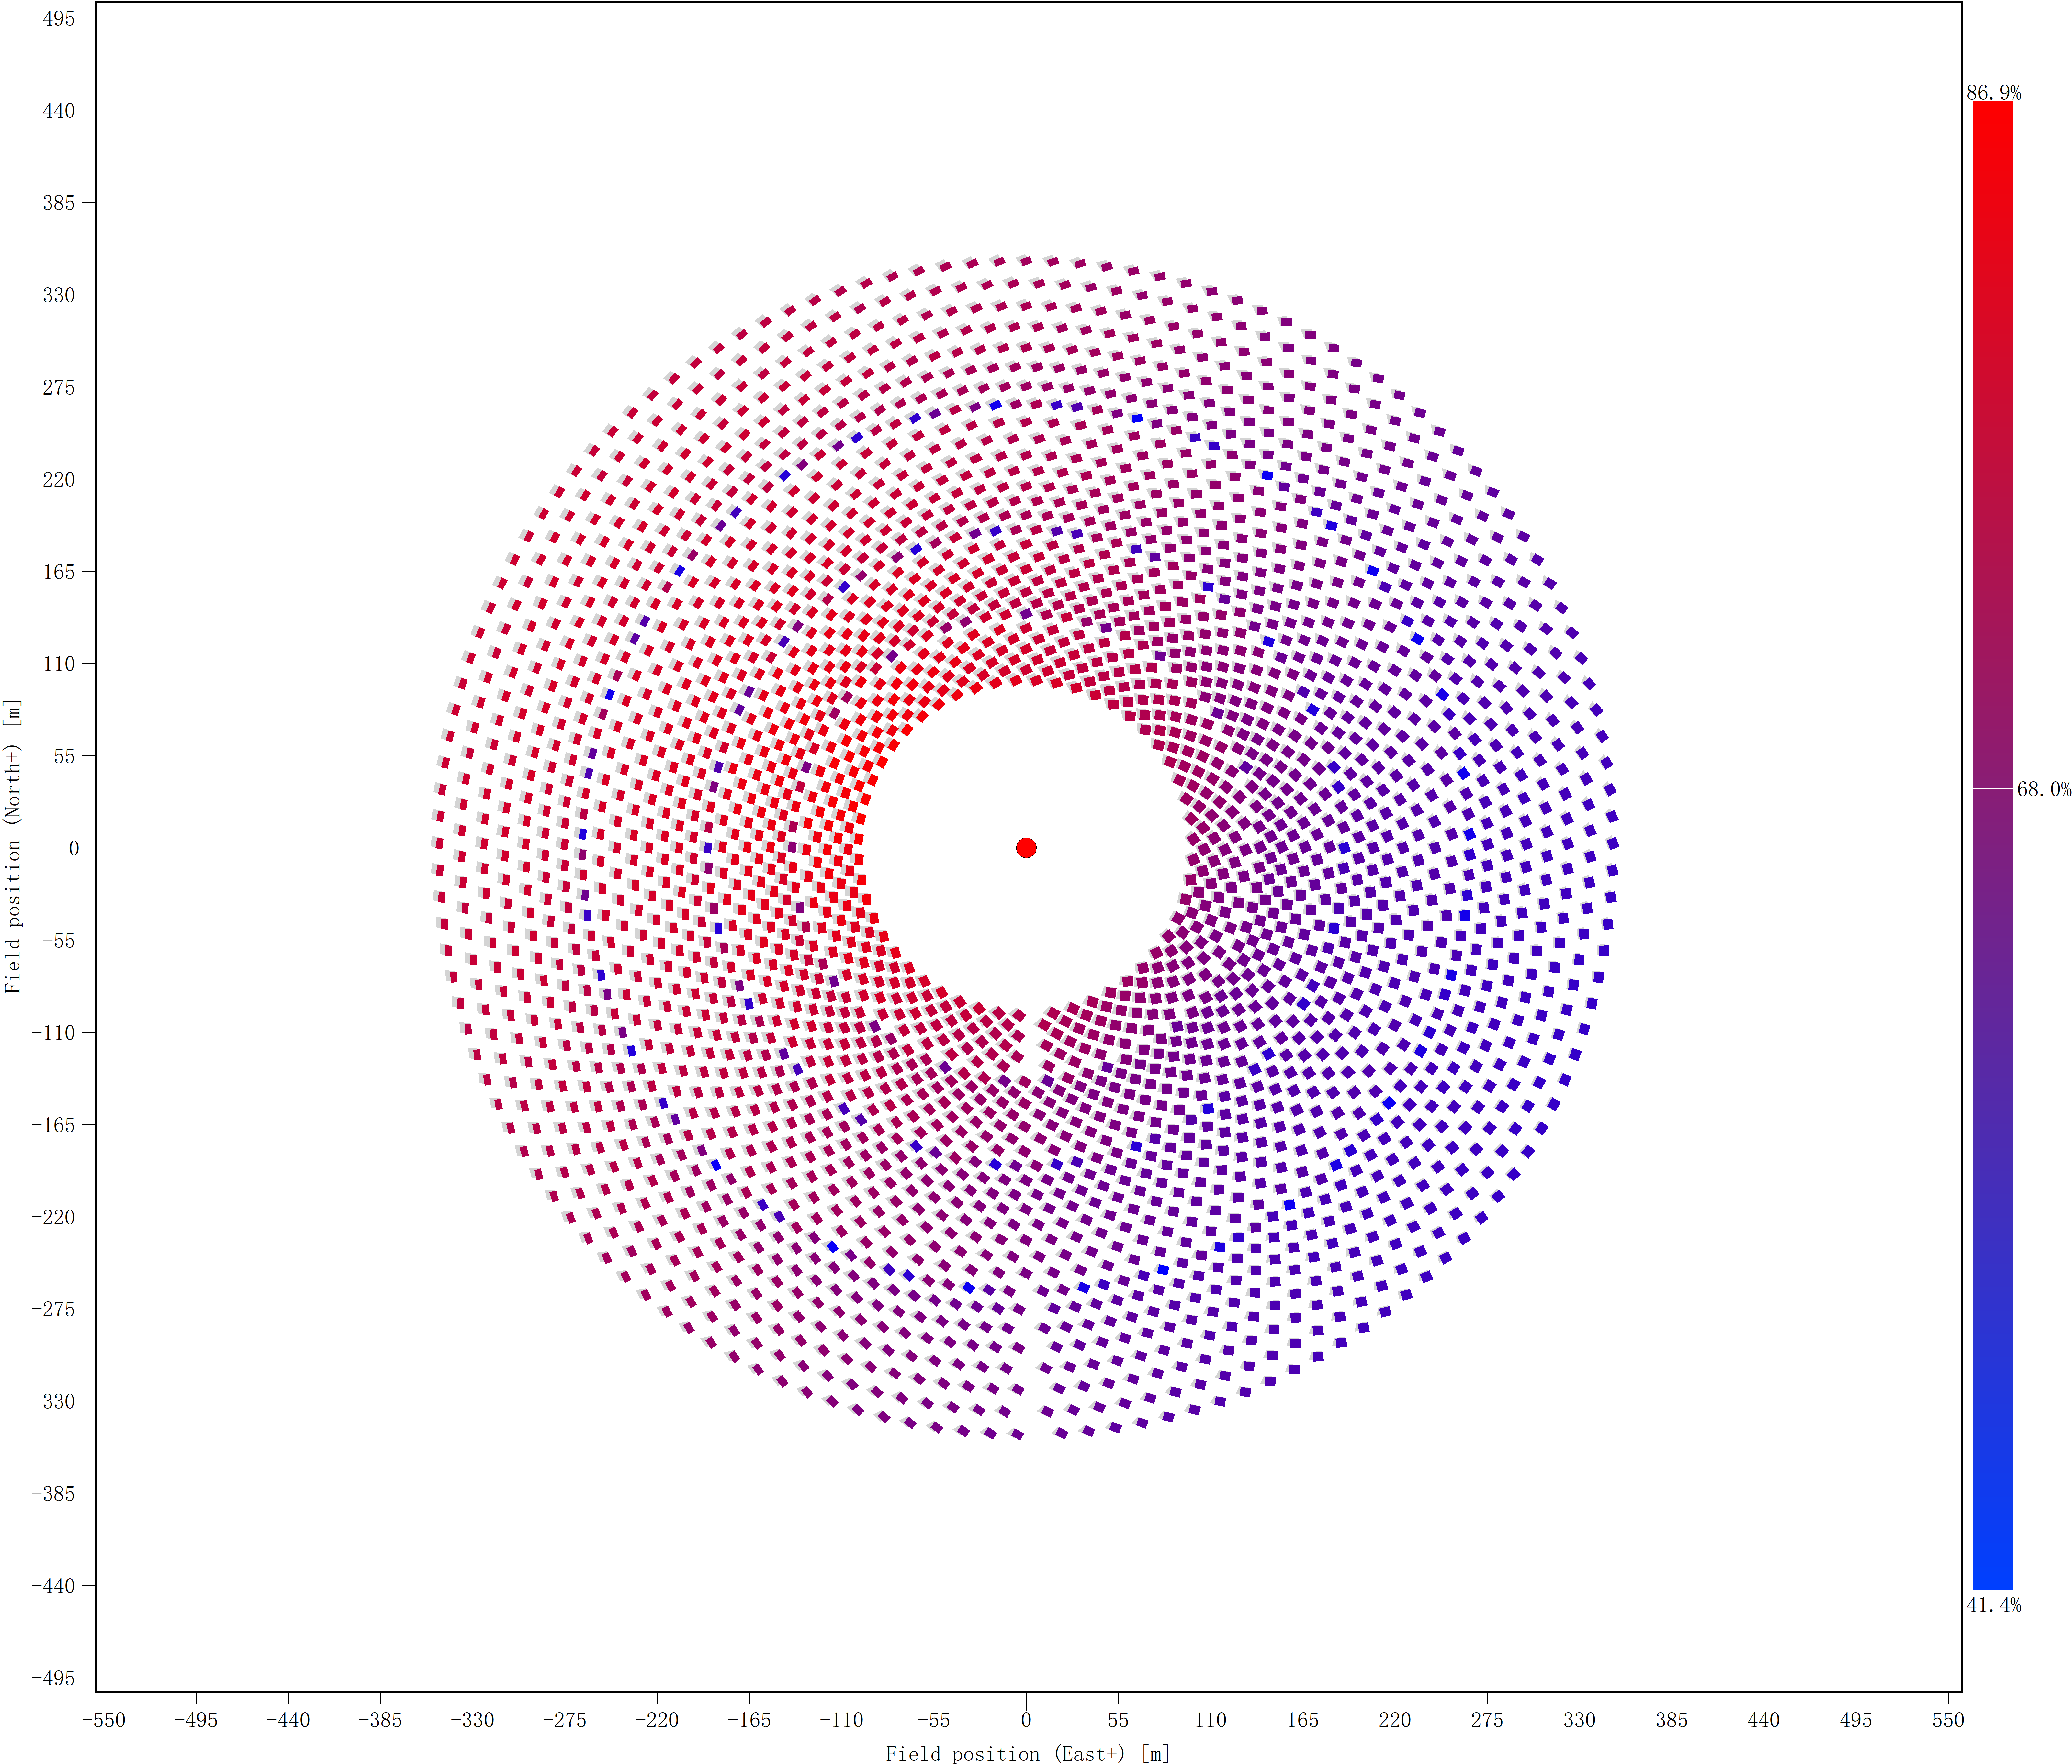
\includegraphics[width=\textwidth,height=.82\textwidth]{figures/2682夏至.png}%这个tmd大小不一样阿
\end{subfigure}
\begin{subfigure}[b]{.49\textwidth}
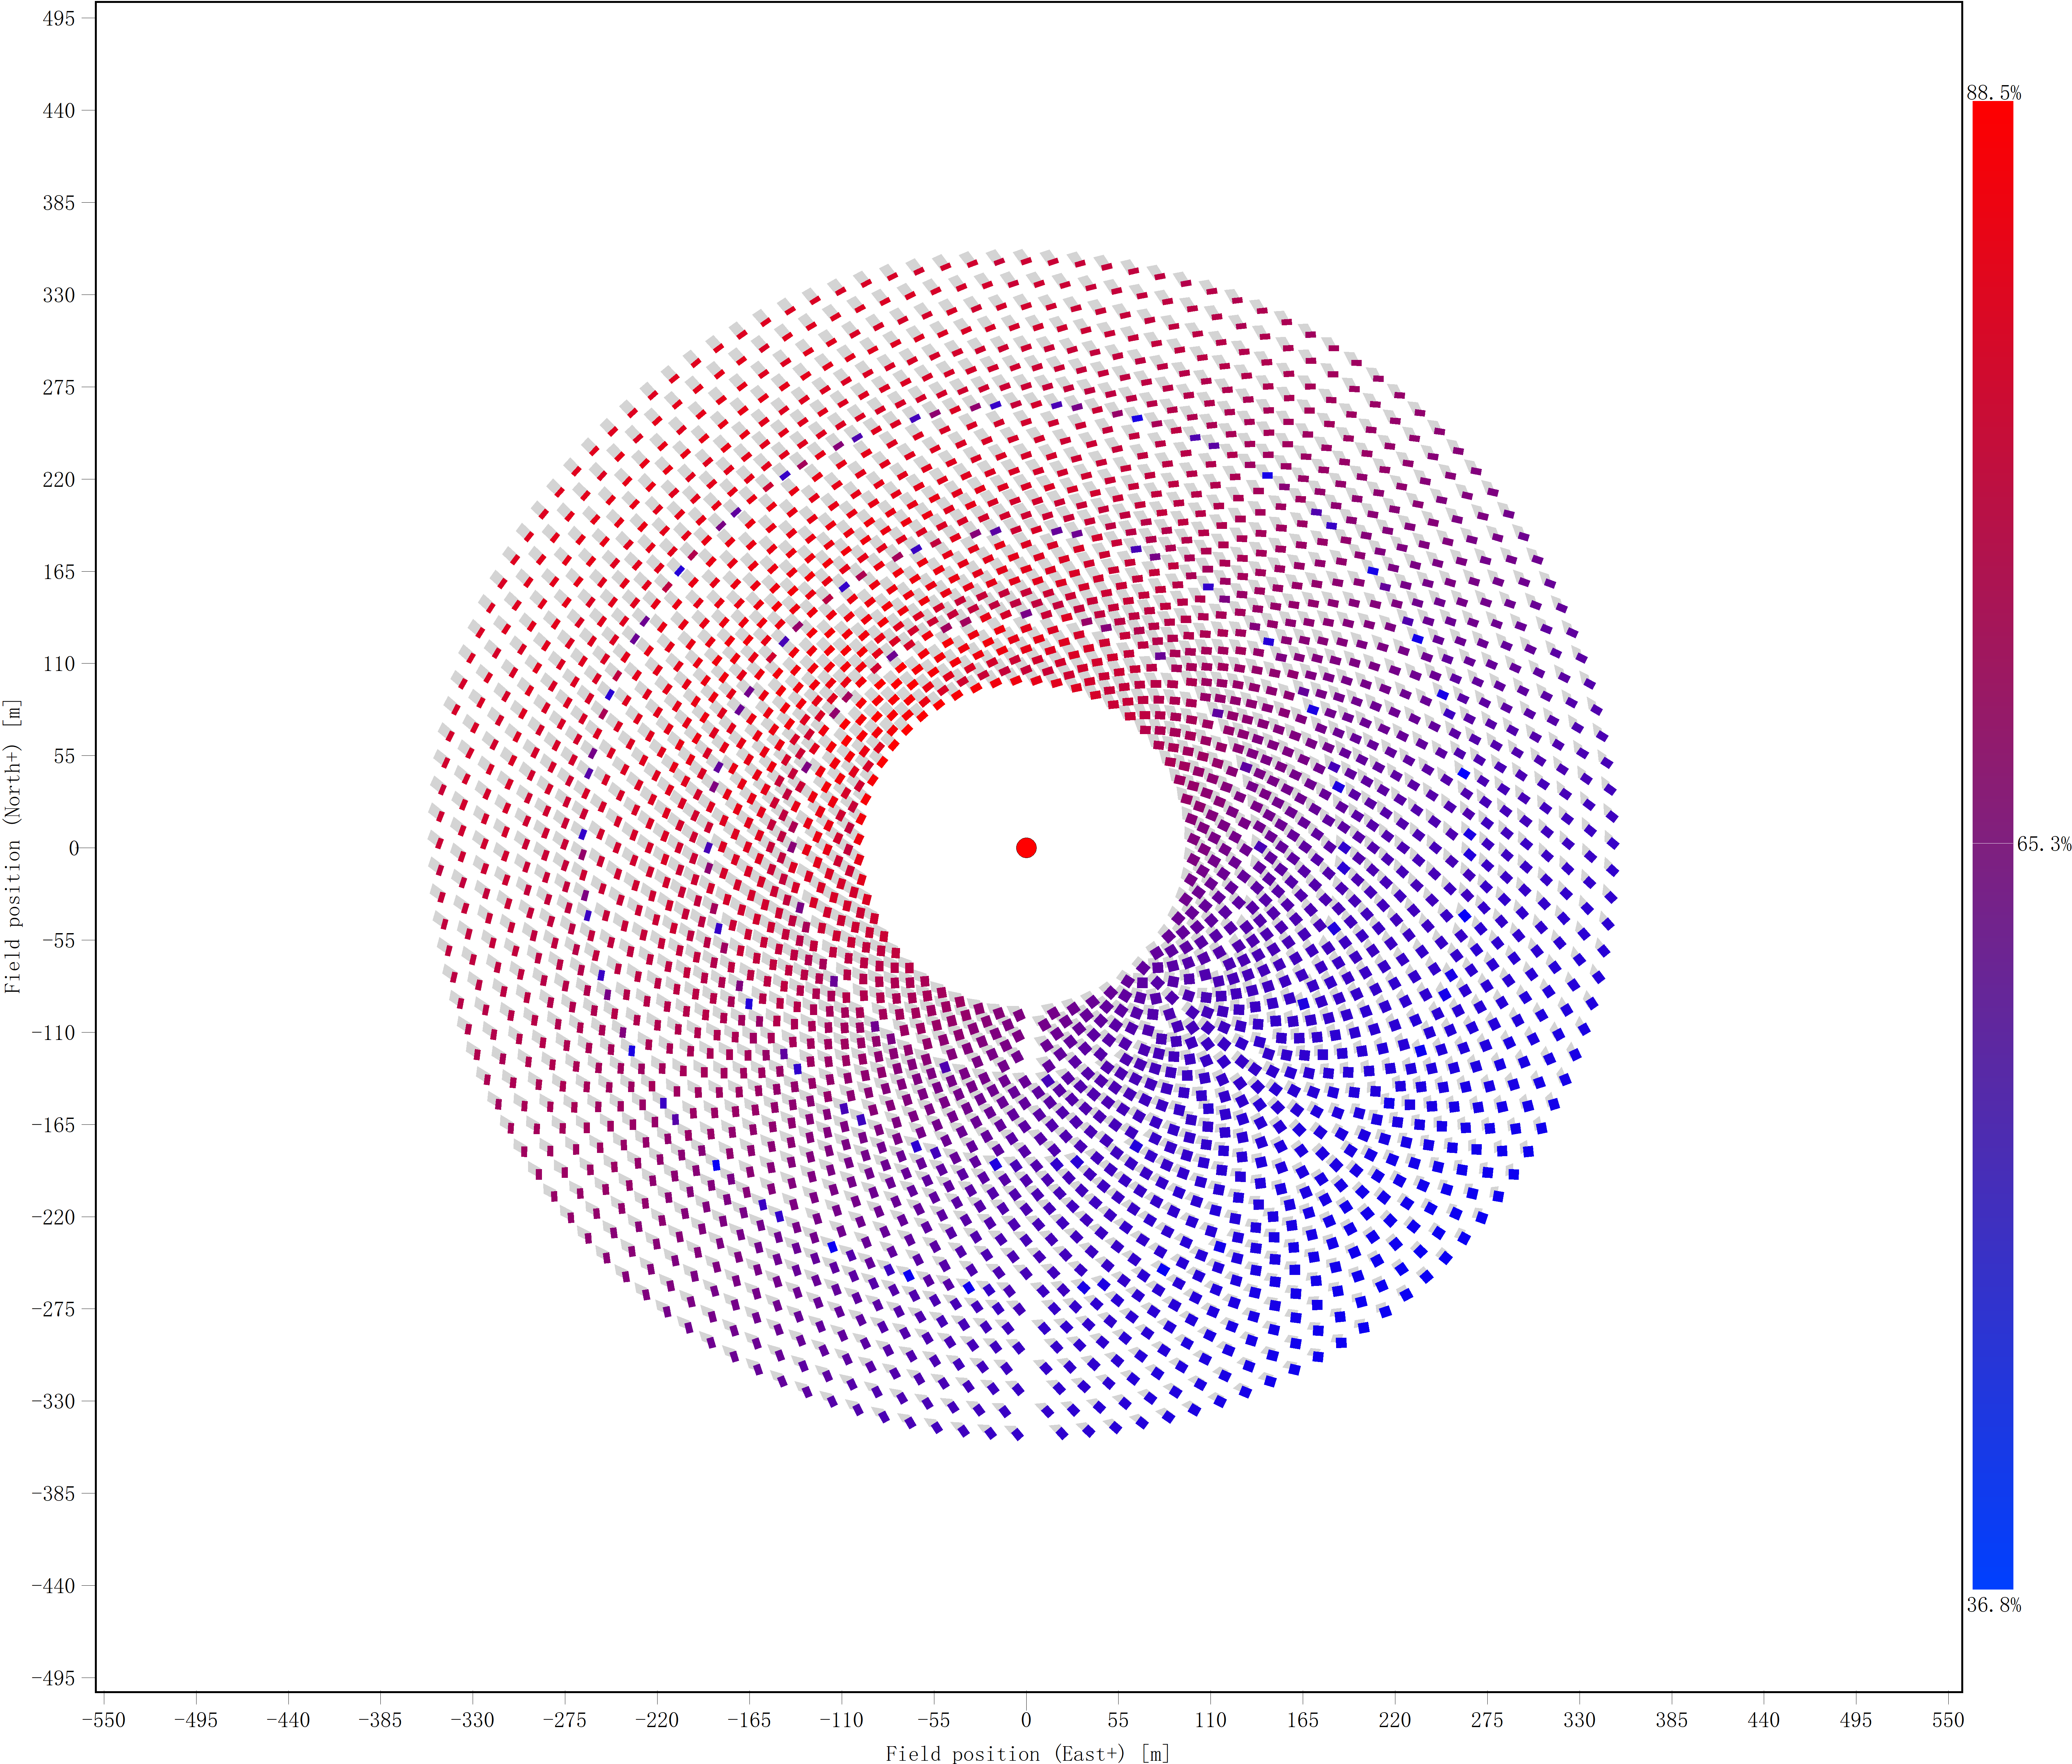
\includegraphics[width=\textwidth]{figures/2682秋分.png}
\end{subfigure}
\begin{subfigure}[b]{.49\textwidth}
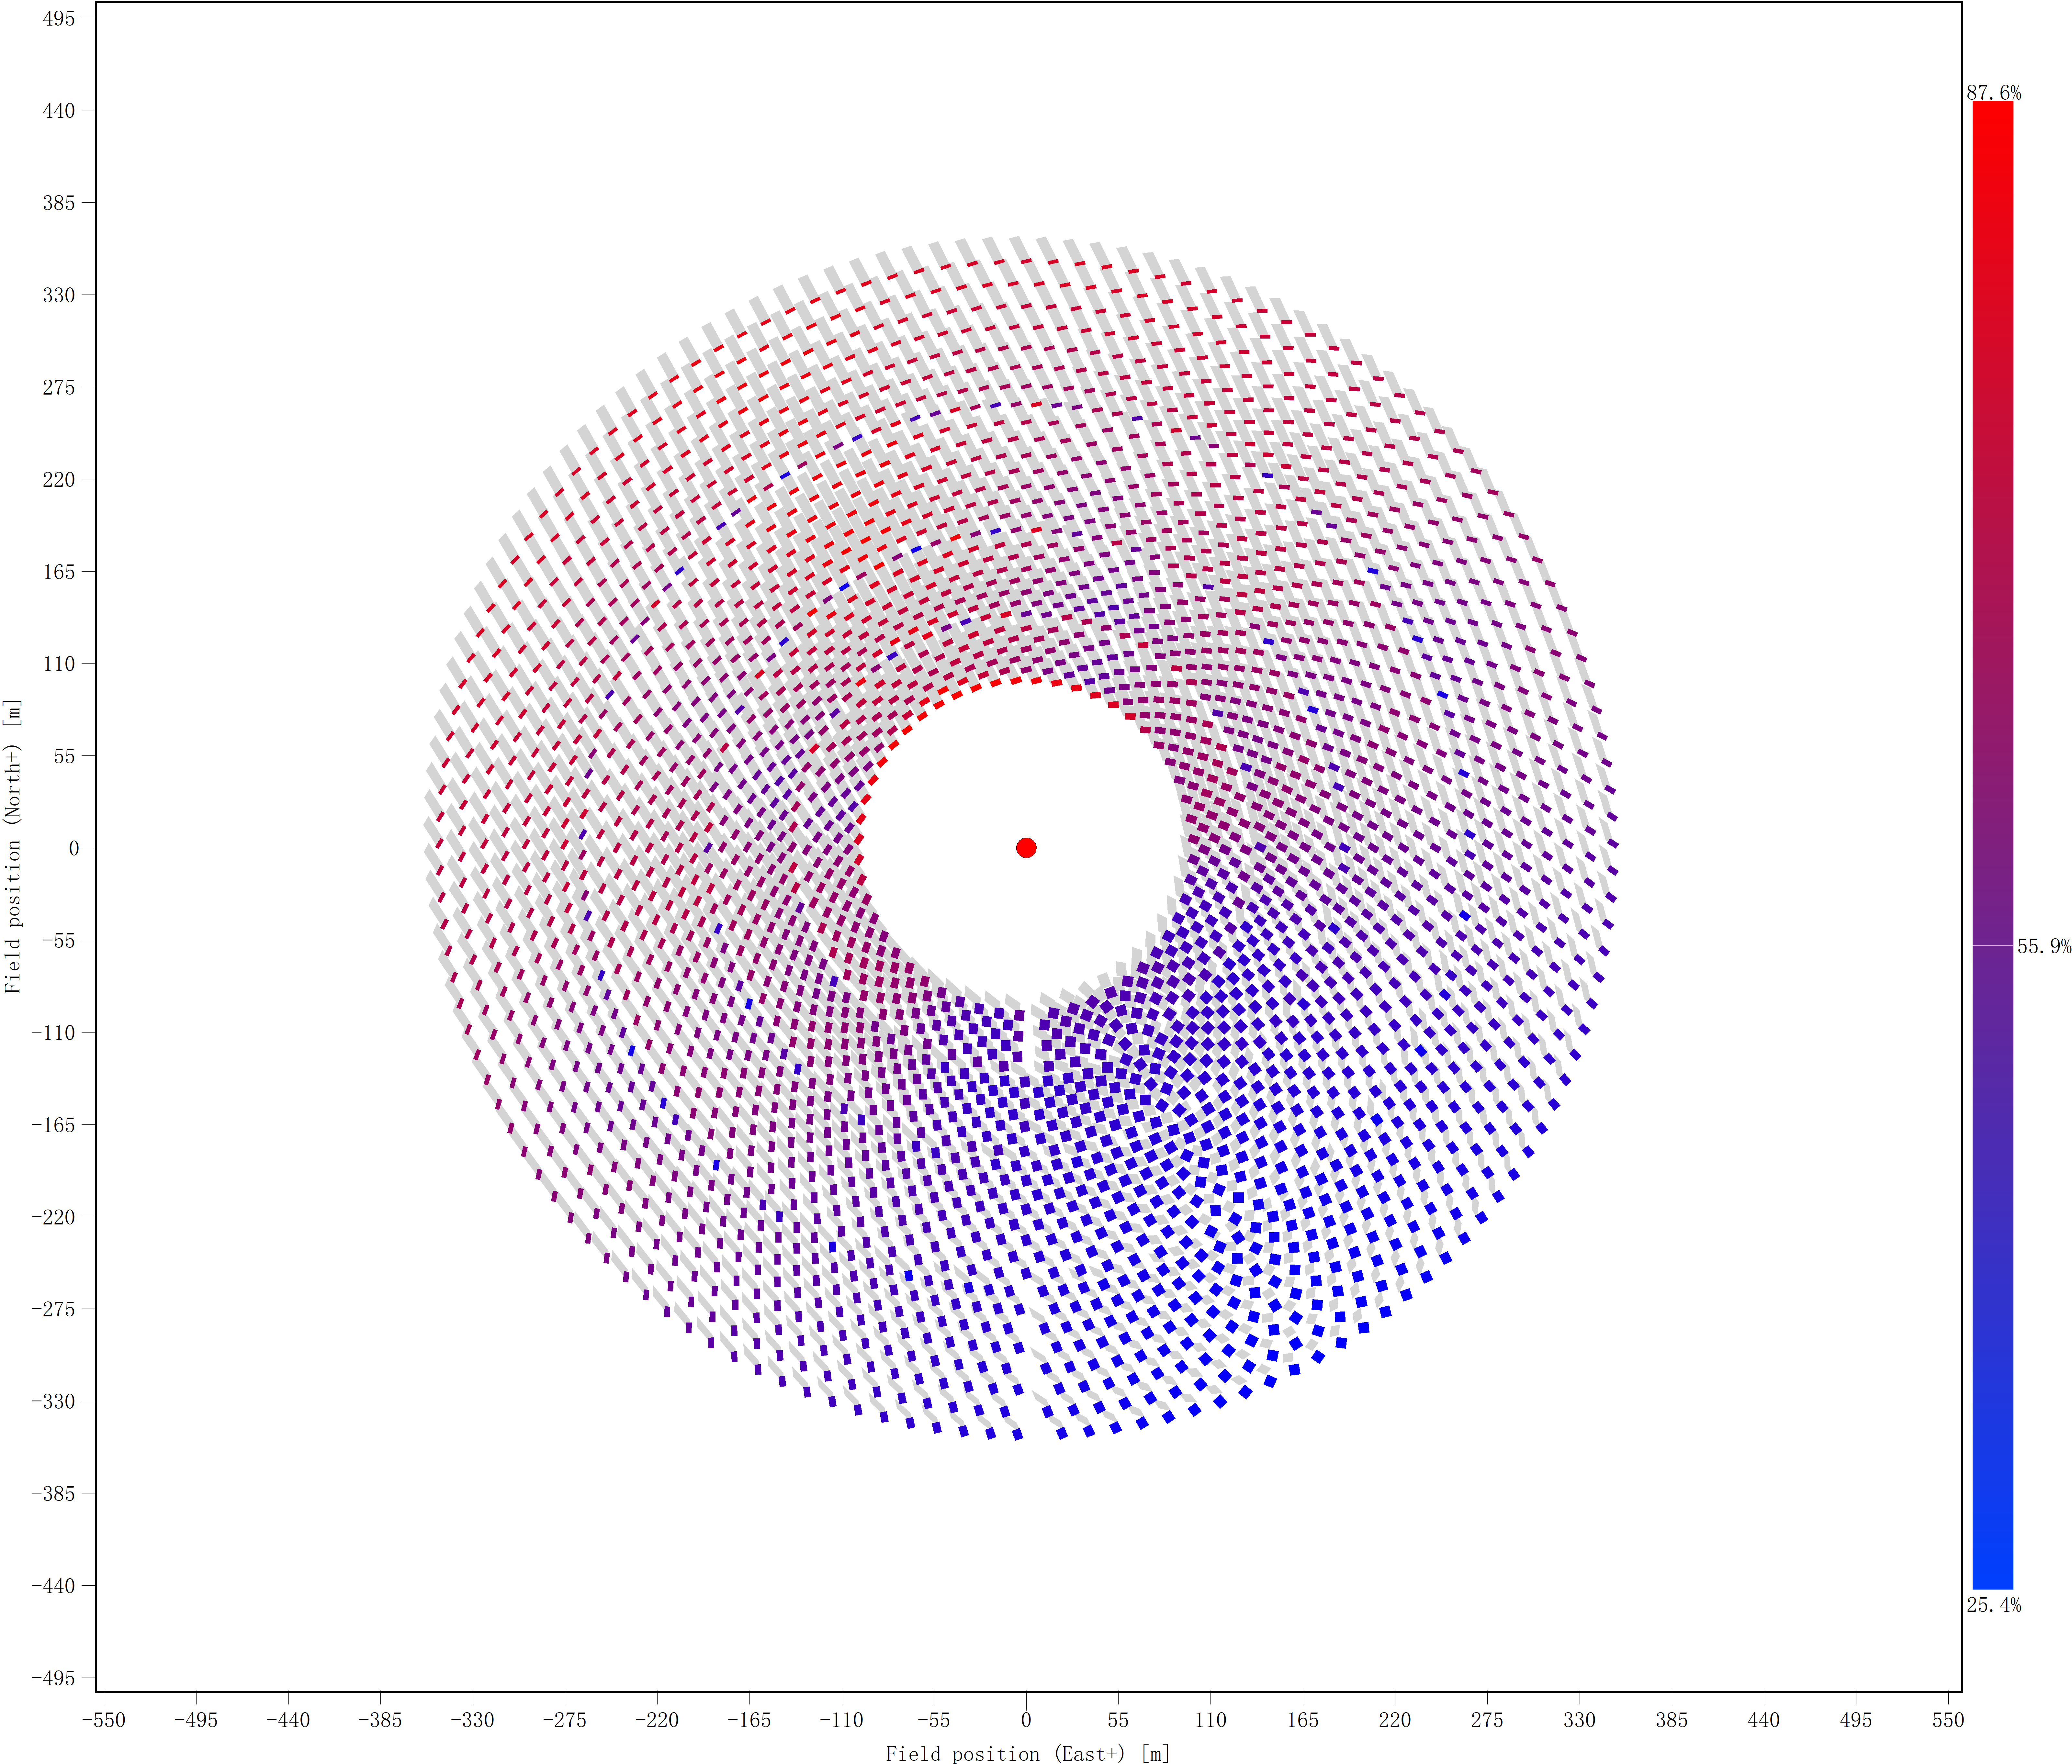
\includegraphics[width=\textwidth]{figures/2682冬至.png}
\end{subfigure}
\caption{优化后镜场四个季度仿真云图}\label{cxqd}
\end{figure}
\item 在Performance Simulation界面对60个相应时间点的模型进行运行,得出有关阴影遮挡效率、余弦效率、截断效率及额定输入热功率的数据,最后对所得数据进行处理,该镜场平均光学效率及输出功率见表\ref{s1},年平均光学效率及输出功率表见表\ref{s2},设计参数见表\ref{s3},吸收塔的位置坐标、定日镜尺寸、安装高度、位置坐标保存在 result2.xlsx文件中,详见附件。 
\end{enumerate}
\begin{table}[H]
\centering
\caption{问题二每月21日平均光学效率及输出功率}
\label{s1}\resizebox{\textwidth}{!}{
\begin{tabular}{@{}cccccc@{}}
\toprule
日期 & 平均光学效率 & 平均余弦效率 & 平均阴影遮挡效率 & 平均截断效率 & 单位面积镜面平均输出热功率 ($kW/m^2$) \\ \midrule
1月21日  & 0.580436776 & 0.704200 & 0.94226  & 0.9848   & 0.553760030 \\
2月21日  & 0.540413194 & 0.669980 & 0.92088  & 0.9861   & 0.549311480 \\
3月21日  & 0.595651021 & 0.735100 & 0.92313  & 0.9882   & 0.622516170 \\
4月21日  & 0.655364734 & 0.764975 & 0.97888  & 0.9853   & 0.698563461 \\
5月21日  & 0.681784241 & 0.778075 & 0.99160  & 0.9948   & 0.721905198 \\
6月21日  & 0.684903026 & 0.780125 & 0.99275  & 0.9956   & 0.726592725 \\
7月21日  & 0.682423089 & 0.782540 & 0.99088  & 0.9908   & 0.716530862 \\
8月21日  & 0.665817560 & 0.771980 & 0.98176  & 0.9890   & 0.700932469 \\
9月21日  & 0.637805107 & 0.754260 & 0.96172  & 0.9899   & 0.656684296 \\
10月21日 & 0.606832877 & 0.722500 & 0.95702  & 0.9880   & 0.575070065 \\
11月21日 & 0.599601300 & 0.727160 & 0.94025  & 0.9873   & 0.485734129 \\
12月21日 & 0.624031158 & 0.767522 & 0.93018  & 0.9840   & 0.547277295 \\ \bottomrule
\end{tabular}}
\end{table}


\begin{table}[H]
\centering
\caption{问题二年平均光学效率及输出功率表}
\label{s2}\resizebox{\textwidth}{!}{
\begin{tabular}{@{}cccccc@{}}
\toprule
年平均光学效率 & 年平均余弦效率  & 年平均阴影遮挡效率 & 年平均截断效率 & 年平均输出热功率 ($MW$) & 单位面积镜面年平均输出热功率 ($kW/m^2$) \\ \midrule
0.57547 & 0.733489 & 0.9283167 & 0.98079 & 62.6022816    & 0.62957684             \\ \bottomrule
\end{tabular}}
\end{table}
\begin{table}[H]
\centering
\caption{问题二设计参数表}
\label{s3}\resizebox{\textwidth}{!}{
\begin{tabular}{@{}ccccc@{}}
\toprule
吸收塔位置坐标 &
  定日镜尺寸(宽 ×高) &
  定日镜安装高度(m) &
定日镜总面数&
 定日镜总面积($m^2$) \\ \midrule
(4.52465e-7,0)&
  7.3×6.1 &
  6 &
  2233 &
  99435.49 \\ \bottomrule
\end{tabular}}
\end{table}













































\section{问题三模型建立与求解}
\subsection{问题三模型建立}
该问在可以考虑不同定日镜间参数可以不同的情况下,仍先考虑优化定日镜布局。首先考虑定日镜安装高度,增大定日镜安装高度会增大余弦效率、增大阴影遮挡效率,我们仍采用问题二中DELSOL3型布局方式,考虑在区域$k$中的定日镜安装高度为$h_k$,有:

\begin{eqnarray}
h_k\ge\frac{LW}{2} ,\forall k
\end{eqnarray}

则第一个基本区域$h_1$和最后一基本区域定日镜安装高度为$h_n$满足:

\begin{eqnarray}
2\le h_1\le h_n\le6
\end{eqnarray}

对于初始布局,我们可以取各区域安装高度增量$\Delta h$为一定值,并且满足:
\begin{eqnarray}
2+(k-1)\Delta h\le h_{k}\le6-(n-k)\Delta h
\end{eqnarray}

上式使得每个区域的安装高度均不超过下一区域安装高度的最小值,不低于上一区域安装高度的最大值。

在该问中令$n=50$,即将镜场划分为50个不同半径的同心圆环区域,并分别进行区域化的优化,使得满足问题二的约束条件以及安装高度约束的情况下输出单位镜面面积年平均输出热功率。由于在问题二中已经对吸收塔的位置进行了多次迭代优化,所以在问题三中我们使用问题二所得结论,不再对吸收塔位置进行讨论。
\subsection{模型求解}
我们以第一个区域为例,将需要优化的镜场参数输入进软件,进行仿真优化和迭代得到如下镜场年平均光学效率分布云图,如图\ref{yt11}所示:
\begin{figure}[htbp]
\centering
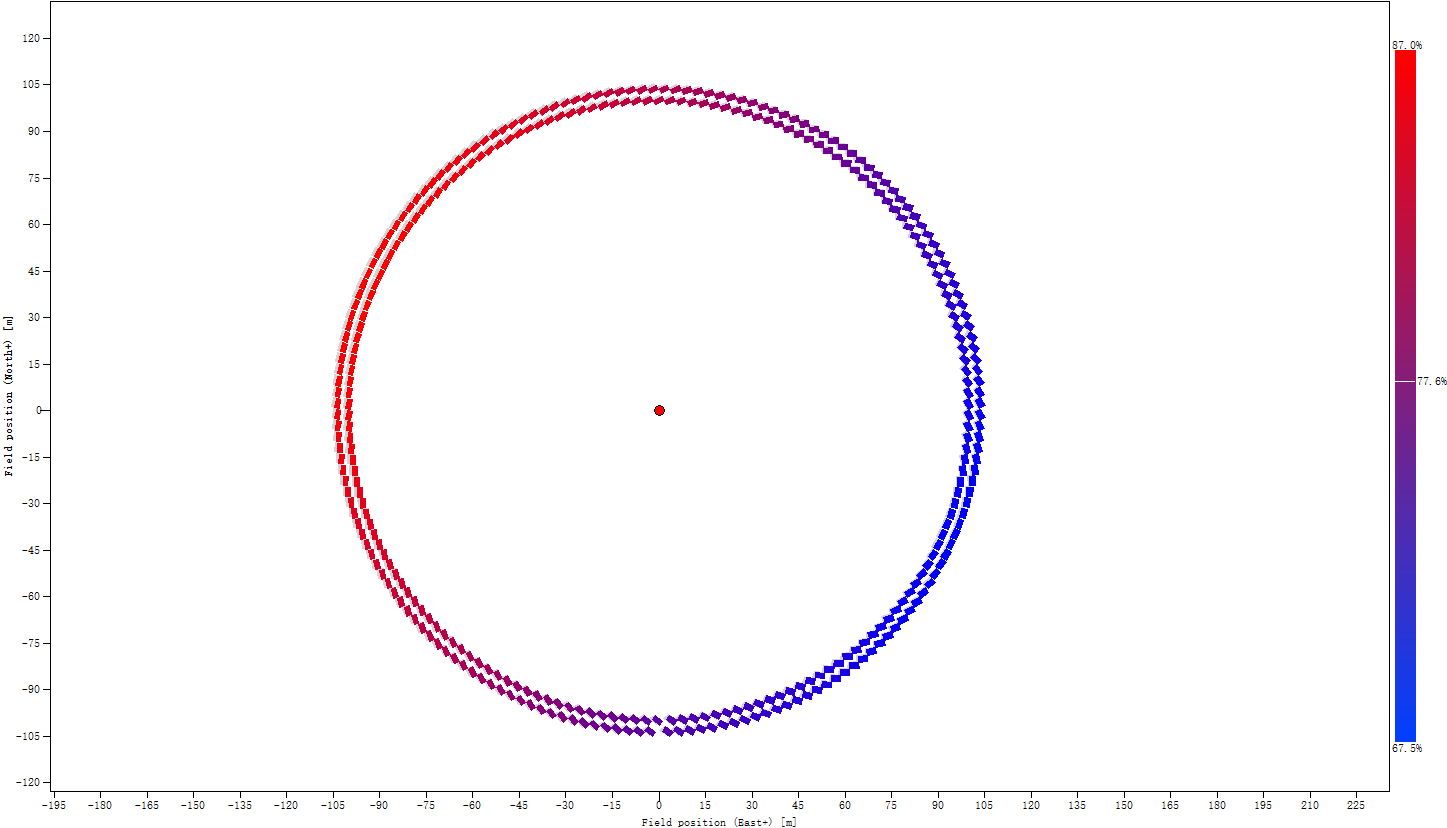
\includegraphics[width=\textwidth]{figures/quan.png}
\caption{第一个区域优化后年平均光学效率分布云图}\label{yt11}
\end{figure}


























\section{模型评价}
\subsection{模型检验}
在问题一中建立模型并利用蒙特卡洛算法来模拟阴影遮挡效率以及截断效率,对于随机化算法我们需要判断其是否收敛。在蒙特卡洛模拟中,只有当迭代次数足够多时才会收敛到真实值附近,在求解过程中选取的点数量为$3\times 10^4$个点,为验证其结果可靠性,随机选取两个存在阴影遮挡损失的定心镜,画出选取的点的数量与计算的阴影遮挡效率的关系,判断算法是否收敛。同理对于截断效率,也随机取两定心镜,其中迭代次数与所求效率值如图\ref{mxjy}:

\begin{figure}[H]
\centering
\begin{subfigure}[b]{.49\textwidth}
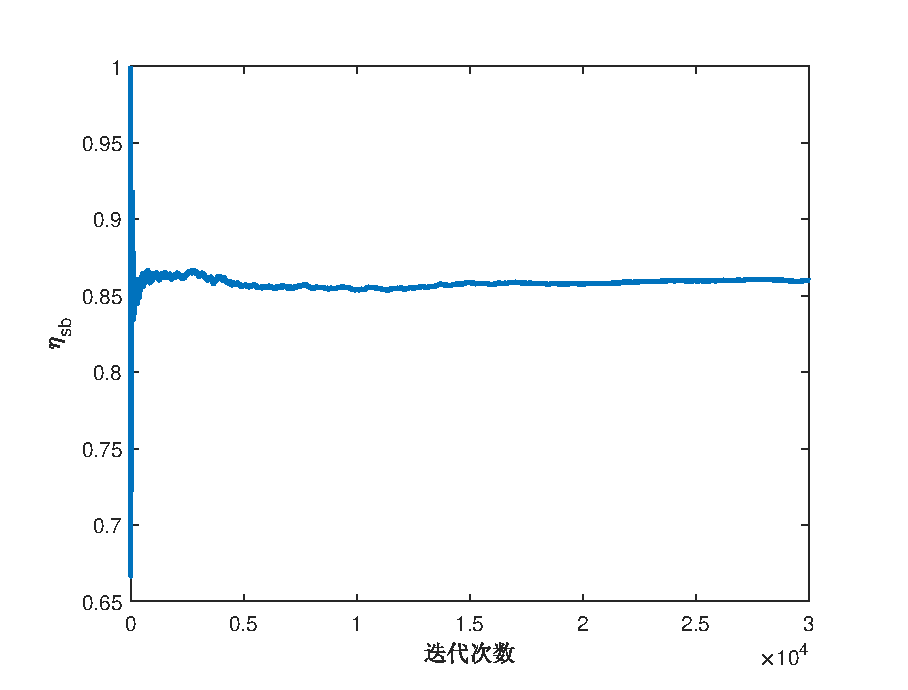
\includegraphics[width=\textwidth]{figures/遮挡模型检验.eps}
\end{subfigure}
\begin{subfigure}[b]{.49\textwidth}
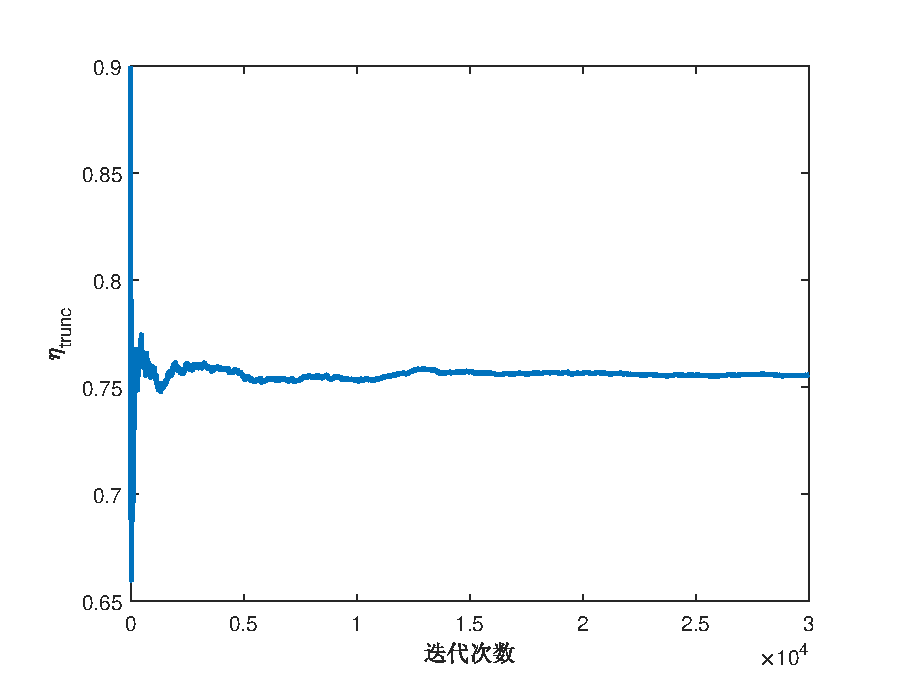
\includegraphics[width=\textwidth]{figures/截断模型检验.eps}
\end{subfigure}
\caption{模型检验}\label{mxjy}
\end{figure}

可以发现在迭代次数达到$1.5\times 10^4$时结果基本收敛,因此可以认为该算法模拟得到的各效率值等于真实值。

\subsection{模型优点}
\begin{itemize}
	\item 建立了镜面坐标系,能够更方便地进行求解。
	\item 我们在求解阴影遮挡损失时考虑到阴影可能并不规则,利用蒙特卡洛模拟合理地简化了计算量。
	\item 利用SolarPILOT软件进行仿真优化比编写代码求解方式效率更高,结果可信度更高。
\end{itemize}
\subsection{模型缺点}
\begin{itemize}
	\item 使用蒙特卡洛模拟时三部分阴影遮挡面积可能存在重叠部分,使得计算结果可能并不准确。建立光锥坐标系利用蒙特卡洛方法与使HFCAL方法计算截断效率相比效率更低,并且精确度不能得到保证。
	\item DELSOL3型镜场分布模型在远离吸收塔过程中,土地利用率迅速减小,不具有普适性。
	\item SolarPILOT软件所提供的经纬度数据与题中所给数据略有偏差,仿真结果存在一定误差。
\end{itemize}










\clearpage

% \begin{eqnarray}
% \begin{matrix}
%  \max T=\sum_j\sum_it_{ij}\\
% \bm{s.t.} \left\{\begin{matrix}
%  i\in V\\
% j\in V
% \end{matrix}\right.
% \end{matrix}
% \end{eqnarray}

% \begin{table}[!h]
%     \caption{问题3结果}
% \label{dc9}
%     \centering
%     \begin{threeparttable}          %这行要添加
    
    
    
%       \begin{tabular}{lcc}
% \toprule
% 改变的线路&  新增的货量&  改变后线路平均负荷率 \\ \midrule
% $DC36\to DC4\tnote{1}$   & 83242  & 98.4$\%$  \\\bottomrule
% \end{tabular}



%          \begin{tablenotes}    %这行要添加, 从这开始
%         \footnotesize               %这行要添加
%         \item[1] 该路线为新增路线,仅在第2、3、8、9天运行。
%       \end{tablenotes}            %这行要添加
%     \end{threeparttable}       %这行要添加,到这里结束
%   \end{table}





















%参考文献
% \clearpage
\begin{thebibliography}{99}%宽度9
\bibitem{x}
{\it 基于光学效率的塔式电站镜场布局优化设计研究}.
\newblock 硕士, 合肥工业大学, 2018.


\bibitem{xx}
Xiudong Wei, Zhenwu Lu, Zi~Lin, Hongxin Zhang, and Zhengguo Ni.
\newblock Optimization procedure for design of heliostat field layout of a
  {1MWe} solar tower thermal power plant.
\newblock page 684119, Beijing, China, November 2007.

\bibitem{xxx}
 丁婷婷 and  祝雪妹.
\newblock {\it 塔式系统圆形镜场中余弦效率分布的研究}.
\newblock {\it 科学技术与工程}, 12(31):8406--8410+8433, 2012.
{\textless}北大核心{\textgreater}.

\bibitem{xxxx}
 丁琦,  曾智勇,  陈武忠,  周传华,  王志峰, and  郭明焕.
\newblock {\it 一种定日镜场有效镜面面积的评估方法}.
\newblock {\it 太阳能学报}, 42(9):184--189, 2021.
\newblock {\textless}北大核心, EI, CSCD{\textgreater}.

\bibitem{xxxxx}
刘建兴 .
\newblock {\it
  塔式光热电站光学效率建模仿真及定日镜场优化布置}.
\newblock 硕士, 兰州交通大学, 2022.

\bibitem{xxxxxx}
 宓霄凌,  王伊娜,  李建华, and  李心.
{\it 塔式太阳能热发电站镜场设计分析}.
\newblock {\it 太阳能}, (6):61--65, 2016.


\bibitem{xxxxxxx}
 张国勋 and  饶孝枢.
{\it 塔式太阳能聚光系统太阳影象方程}.
\newblock {\it 太阳能学报}, (2):172--178, 1982.


\bibitem{xxxxxxxx}
 张宏丽 and  王树群.
{\it 塔式电站中定日镜尺寸的选择}.
\newblock {\it 沈阳工程学院学报(自然科学版)}, 13(3):199--203,
  2017.


\bibitem{xxxxxxxxx}
 程小龙,  尹延国, and  马少波.
{\it 塔式电站定日镜场布局的优化设计研究}.
\newblock {\it 能源与环境}, (2):64--66+70, 2018.


\bibitem{xxxxxxxxxx}
 胡叶广.
\newblock {\it
  塔式太阳能热发电系统的多级反射式聚光镜场的研究}.
\newblock 博士, 哈尔滨工业大学, 2018.


\bibitem{xxxxxxxxxxx}
 赵茜.
\newblock {\it 塔式太阳能热电系统镜场调度的优化}.
\newblock 硕士, 浙江大学, 2017.


\bibitem{xxxxxxxxxxxx}
 邓立宝,  吴怡然, and  郭苏.
\newblock {\it 基于分解多目标进化的椭圆定日镜场布局}.
\newblock {\it 郑州大学学报(工学版)}, 41(5):37--43, 2020.
{\textless}北大核心{\textgreater}.

\bibitem{xxxxxxxxxxxxx}
 高博,  刘建兴,  孙浩, and  刘二林.
\newblock {\it 基于自适应引力搜索算法的定日镜场优化布置}.
\newblock {\it 太阳能学报}, 43(10):119--125, 2022.
\newblock {\textless}北大核心, EI, CSCD{\textgreater}.
\bibitem{z} SolarPILOT | Concentrating Solar Power | NREL. \url{https://www.nrel.gov/csp/solarpilot-background.html} (accessed 2023-09-10).


\end{thebibliography}

 \clearpage
%附录
\begin{appendices}


\section*{附件列表}
\begin{lstlisting}[language=html]
code
├─ result2.xlsx
├─ 第一问.mlx
├─ 计算dHR.py
├─ 计算DNI.py
├─ 计算余弦效率.py
├─ 计算大气透射率 .py
└─ 计算影子长度 .py
\end{lstlisting}
\section{问题一Python代码}
\begin{lstlisting}[language=python]
#计算dHR
import csv
import math


with open('附件1.csv', mode='r') as csv_file, open('新文件1.csv', mode='w', newline='') as new_csv_file:
    csv_reader = csv.reader(csv_file)
    csv_writer = csv.writer(new_csv_file)


    header = next(csv_reader)

    csv_writer.writerow(['X坐标', 'Y坐标', 'S'])


    for row in csv_reader:
        x = float(row[0])
        y = float(row[1])
        s = math.sqrt(x ** 2 + y ** 2 + 76 ** 2)
        csv_writer.writerow([x, y, s])
#计算DNI
import math


D_values = [-59, -28, 0, 31, 61, 92, 122, 153, 184, 214, 245, 275]
ST_values = [9, 10.5, 12, 13.5, 15]

for D in D_values:
    for ST in ST_values:
        SINA = math.sin(2 * math.pi * (D / 365)) * math.sin((2 * math.pi / 360) * 23.45)
        COSA = math.sqrt(1 - SINA**2)
        COSW = math.cos((math.pi / 12) * (ST - 12))
        SINas = COSA * math.cos(math.radians(39.4)) * COSW + SINA * math.sin(math.radians(39.4))
        DNI = 1.366 * (0.34981 + 0.5783875 * math.exp(-0.275745 / SINas))
        print(f"D = {D}, ST = {ST}, DNI = {DNI}")
#计算大气透射率
import math


D_values = [-59, -28, 0, 31, 61, 92, 122, 153, 184, 214, 245, 275]
ST_values = [9, 10.5, 12, 13.5, 15]

for D in D_values:
    for ST in ST_values:
        SINA = math.sin(2 * math.pi * (D / 365)) * math.sin((2 * math.pi / 360) * 23.45)
        COSA = math.sqrt(1 - SINA**2)
        COSW = math.cos((math.pi / 12) * (ST - 12))
        SINas = COSA * math.cos(math.radians(39.4)) * COSW + SINA * math.sin(math.radians(39.4))
        DNI = 1.366 * (0.34981 + 0.5783875 * math.exp(-0.275745 / SINas))
        print(f"D = {D}, ST = {ST}, DNI = {DNI}")
#计算影子长度
import math


D_values = [-59, -28, 0, 31, 61, 92, 122, 153, 184, 214, 245, 275]
ST_values = [9, 10.5, 12, 13.5, 15]

for D in D_values:
    for ST in ST_values:
        SINA = math.sin(2 * math.pi * (D / 365)) * math.sin((2 * math.pi / 360) * 23.45)
        COSA = math.sqrt(1 - SINA**2)
        COSW = math.cos((math.pi / 12) * (ST - 12))
        SINas = COSA * math.cos(math.radians(39.4)) * COSW + SINA * math.sin(math.radians(39.4))
        COSas=math.sqrt(1-SINas**2)
        TANas=SINas/COSas
        L=84/TANas
        print(f"D = {D}, ST = {ST}, 影子长度 = {L}")
#计算余弦效率
import math
import csv

x_values = []
y_values = []

with open('附件.csv', 'r') as csv_file:
    csv_reader = csv.reader(csv_file)
    next(csv_reader)
    for row in csv_reader:
        x_values.append(float(row[0]))
        y_values.append(float(row[1]))

D_values = [-59, -28, 0, 31, 61, 92, 122, 153, 184, 214, 245, 275]
ST_values = [9, 10.5, 12, 13.5, 15]


cosine_efficiency = {}


for D in D_values:
    for ST in ST_values:
        SINA = math.sin(2 * math.pi * (D / 365)) * math.sin((2 * math.pi / 360) * 23.45)
        COSA = math.sqrt(1 - SINA ** 2)
        COSW = math.cos((math.pi / 12) * (ST - 12))
        cos_efficiency_values = []  
        for x, y in zip(x_values, y_values):
            SINas = COSA * math.cos(math.radians(39.4)) * COSW + SINA * math.sin(math.radians(39.4))
            COSas = math.sqrt(1 - SINas ** 2)
            COSgs = (SINA - SINas * math.sin(math.radians(39.4))) / (
                    math.sqrt(1 - SINas ** 2) * math.cos(math.radians(39.4)))
            COSAA = (SINA - SINas * math.sin(math.radians(39.4))) / COSas * math.cos(math.radians(39.4))
            SINAA = math.sqrt(1 - COSAA ** 2)
            COS2O = (-x * math.sqrt(1 - SINas ** 2) * SINAA - y * math.sqrt(1 - SINas ** 2) * math.sqrt(
                1 - SINAA ** 2) + 80 * SINas) / math.sqrt(x ** 2 + y ** 2 + 80 ** 2)
            COSO = math.sqrt((1 + COS2O) / 2)
            cos_efficiency_values.append(COSO)

     
        key = f'D{D}_ST{ST}'
        cosine_efficiency[key] = cos_efficiency_values

with open('结果1.csv', 'w', newline='') as result_file:
    csv_writer = csv.writer(result_file)
    header = ['D', 'ST'] + [f'余弦效率_{i}' for i in range(1, len(cosine_efficiency['D-59_ST9']) + 1)]
    csv_writer.writerow(header)

    for D in D_values:
        for ST in ST_values:
            key = f'D{D}_ST{ST}'
            row_data = [D, ST] + cosine_efficiency[key]
            csv_writer.writerow(row_data)

print("数据已保存到结果.csv文件中。")

\end{lstlisting}
\section{问题一MATLAB代码}
\begin{lstlisting}[language=Matlab]
A=xlsread("附件.xlsx");%xy坐标数据

ST=[9 10.5 12 13.5 15]; % 当地时间
D=[310,341,0,31,61,92,122,153,184,224,255,285]; % 春分起天数
phi=39.4*pi/180; % 纬度
omega=pi*(ST-12)/12; % 太阳时角

% 预分配内存
alphas = zeros(length(D), length(ST));
gamas = zeros(length(D), length(ST));

det = asin(sin(2*pi*D/365)*sin(2*pi/360*23.45)); % 赤纬角

for i = 1:length(det)
    deta = det(i);
    alphas(i,:) = asin(cos(deta).*cos(phi).*cos(omega) + sin(deta).*sin(phi)); % 高度角
    gamas(i,:) = real(acos((sin(deta) - sin(alphas(i,:)).*sin(phi)) ./ (cos(alphas(i,:)).*cos(phi)))); % 方位角
end
%入射光线单位向量
ga=cos(alphas).*sin(gamas);
gb=cos(alphas).*cos(gamas);
gc=sin(alphas);

DNI=1.366*(0.4237-0.00821*9+(0.5055+0.00595*3.5*3.5).*exp(-(0.2711+0.01858*0.25)./sin(alphas)));%DNI
%z方向为-80
z = -80 * ones(size(A, 1), 1);
Rz=[A,z];
%镜面坐标系下z轴方向向量
zj=-(Rz + repmat(i, size(A, 1), 1)) / 2 ;
%两个z轴间夹角EH
EH = atan((zj(:,1).^2+zj(:,2).^2)./zj(:,3)) ;
%变换后z轴的投影与正半轴夹角
AH = atan(zj(:,2)./zj(:,1)) ;
l=88./tan(alphas);

%初始化参数
n_points = 1000; % 在每个镜面上随机选取点进行模拟
n_mirrors = 1745;
%坐标
mirror_coords = A;
% 初始化阴影遮挡效率数组
eta_sb = zeros(n_mirrors, 60);
%太阳光向量I遍历
for m=1:12
    for n=1:5
        I=[ga(m,n),gb(m,n),gc(m,n)];

        % 对每一对镜面组合进行迭代
        for j = 1:n_mirrors
            k=0;
            for i=1:n_mirrors
                if i == j
                    continue;
                end

                % 获取镜面i和镜面j的坐标
                x_i = mirror_coords(i, 1);
                y_i = mirror_coords(i, 2);
                x_j = mirror_coords(j, 1);
                y_j = mirror_coords(j, 2);
                sah=sin(AH(i));
                cah=cos(AH(i));
                seh=sin(EH(i));
                ceh=cos(EH(i));
                sahj=sin(AH(j));
                cahj=cos(AH(j));
                sehj=sin(EH(j));
                cehj=cos(EH(j));
                % 计算转换矩阵
                T_i = [-sah,-cah*ceh,cah*seh;cah,-sah*ceh,sah*seh;0,seh,ceh];
                T_j = [-sahj,-cahj*cehj,cahj*sehj;cahj,-sahj*cehj,sahj*sehj;0,sehj,cehj];

                % 镜面i和镜面j中心在H0下的坐标
                O_i = [x_i, y_i, 4];
                O_j = [x_j, y_j, 4];

                % 对每一个镜面i上的点进行迭代

                % 在镜面i上随机选择一个点(这里镜面大小为6x6)

                H1_Hi = [(rand(n_points,2)*2-1)*3,zeros(n_points,1)];

                % 将 H1 从 Hi 转换到 H0
                H1_H0 = T_i * H1_Hi' + O_i';

                % 再将 H1 从 H0 转换到 Hj
                H1_Hj = T_j \ (H1_H0 - O_j');

                % 光线向量在 H0 下迭代
                V_H0 = I;

                % 将光线向量从 H0 转换到 Hj
                V_Hj = T_j\ V_H0';

                % 计算落在镜面j上的坐标 H2
                a = V_Hj(1); b = V_Hj(2); c = V_Hj(3);
                x1 = H1_Hj(1,:); y1 = H1_Hj(2,:); z1 = H1_Hj(3,:);
                t = -z1 / c;
                x2 = x1 + a * t;
                y2 = y1 + b * t;

                % 判断 H2 是否落在镜面j内(这里镜面大小为6x6)
                k=k+length(find(abs(x2) <= 3 & abs(y2) <= 3));
            end
            ii=5*(m-1)+n;%计数器
            eta_sb(j,ii)=1-k/n_points;
        end
    end
end


% 输出结果
disp(eta_sb);


% 初始化参数
n_points = 30000; % 在每个镜面上随机选取30000个点进行模拟
n_mirrors = 1745;
% % %坐标
mirror_coords = A;
tao=(rand(n_points,1)*2-1)*0.00465+pi/2;%tao的值在[pi/2-4.65e-3,pi/2+4.65e-3]之间
sigma=rand(n_points,1)*0.00465;%sigma值在[0,4.65e-3]之间
XY=[(rand(n_points,2)*2-1)*3,zeros(n_points,1)]%H_1的xy坐标
Ss=[sin(sigma).*cos(tao),sin(sigma).*sin(tao),cos(tao)];%向量Ss
eta_t=zeros(n_mirrors,1);
zz=zeros(n_points, n_mirrors);
for i=1:n_mirrors
    x_i = mirror_coords(i, 1);
    y_i = mirror_coords(i, 2);
    X_i = [1 0 0];%x轴向量
    Z_i = [cos(AH(i))*sin(EH(i)) sin(AH(i))*sin(EH(i)) cos(EH(i))];%z轴向量
    Y_i = cross(X_i,Z_i);
    Tt_i=[X_i' Z_i' Y_i'];
    Tt_i=Tt_i/norm(Tt_i); % 转换矩阵
    sah=sin(AH(i));
    cah=cos(AH(i));
    seh=sin(EH(i));
    ceh=cos(EH(i));
    % 计算转换矩阵
    T_i = [-sah,-cah*ceh,cah*seh;cah,-sah*ceh,sah*seh;0,seh,ceh];
    O_i = [x_i, y_i, 4];
    XY_H0 = T_i * XY' + O_i';%H1|HA--H1|H0
    Ss_H0 = Tt_i * Ss';%Ss|HS--Ss|H0
    OAZA = T_i * [0 0 1]';%OAZA|HA--OAZA|H0
    m=Ss_H0(1,:); n = Ss_H0(2,:); l = Ss_H0(3,:);
    x1 = XY_H0(1,:); y1 = XY_H0(2,:); z1 = XY_H0(3,:);
    % 定义目标函数
    FF = @(zz) ((m'.*(zz-z1')./l'+x1').^2+((n'.*(zz)-z1')./l'+y1').^2-49/4).^2;

    % 初始猜测值
    x0 = zeros(n_points, 1) + 88;  % 设置初始值

    % 设置优化选项
    options = optimoptions('lsqnonlin', 'Display', 'off');
    options.Algorithm = 'levenberg-marquardt';
    % 进行非线性最小二乘优化
    [zz(:,i),aa,aaa,saaaa] = lsqnonlin(FF, x0, [], [], options)
    eta_t(:,i)=(length(find(76<=zz(:,i)&zz(:,i)<=4)))/n_points;
end

% 初始化参数
n_points = 30000; % 在每个镜面上随机选取30000个点进行模拟
n_mirrors = 1745;
% % %坐标
mirror_coords = A;
% % 初始化阴影遮挡效率数组
etasb1 = zeros(n_mirrors, 60);
%太阳光向量I遍历
for m=1:12
    for n=1:5
        I=[ga(m,n),gb(m,n),gc(m,n)];

        % 对每一对镜面组合进行迭代
        for j = 1:n_mirrors
            k=0;

            % 获取吸收塔ddd和镜面j的坐标
            x_j = mirror_coords(j, 1);
            y_j = mirror_coords(j, 2);
            sahj=sin(AH(j));
            cahj=cos(AH(j));
            sehj=sin(EH(j));
            cehj=cos(EH(j));
            % 计算转换矩阵
            T_j = [-sahj,-cahj*cehj,cahj*sehj;cahj,-sahj*cehj,sahj*sehj;0,sehj,cehj];

            %镜面j中心在H0下的坐标
            O_j = [zeros(n_points,1)+x_j, zeros(n_points,1)+y_j, zeros(n_points,1)+4];

            % 对每一个吸收塔ddd上的点进行迭代

            % 在吸收塔ddd上随机选点
            H1_H0 = [(rand(n_points,2)*2-1)*3.5 rand(n_points,1)*84];

            % 再将 H1 从 H0 转换到 Hj
            H1_Hj = T_j \( H1_H0' - O_j');

            % 光线向量在 H0 下迭代
            V_H0 = I;

            % 将光线向量从 H0 转换到 Hj
            V_Hj = T_j\ V_H0';

            % 计算落在镜面j上的坐标 H2
            a = V_Hj(1); b = V_Hj(2); c = V_Hj(3);
            x1 = H1_Hj(1,:); y1 = H1_Hj(2,:); z1 = H1_Hj(3,:);
            t = -z1 / c;
            x2 = x1 + a * t;
            y2 = y1 + b * t;

            % 判断 H2 是否落在镜面j内(这里镜面大小为6x6)
            k=k+length(find(abs(x2) <= 3 & abs(y2) <= 3));
            ii=5*(m-1)+n;%计数器
            etasb1(j,ii)=1-k/n_points;
        end
    end
end



% 输出结果
disp(etasb1);

%模型检验
n_points = 30000; % 在每个镜面上选取30000个点进行模拟
n_mirrors = 1745;
%坐标
mirror_coords = A;
% 初始化阴影遮挡效率数组
eta_sb = zeros(n_mirrors, 60);
%太阳光向量I遍历

I=[ga(1,1),gb(1,1),gc(1,1)];

% 对每一对镜面组合进行迭代
i=145;

j=80;
% 获取镜面i和镜面j的坐标
x_i = mirror_coords(i, 1);
y_i = mirror_coords(i, 2);
x_j = mirror_coords(j, 1);
y_j = mirror_coords(j, 2);
sah=sin(AH(i));
cah=cos(AH(i));
seh=sin(EH(i));
ceh=cos(EH(i));
sahj=sin(AH(j));
cahj=cos(AH(j));
sehj=sin(EH(j));
cehj=cos(EH(j));
% 计算转换矩阵
T_i = [-sah,-cah*ceh,cah*seh;cah,-sah*ceh,sah*seh;0,seh,ceh];
T_j = [-sahj,-cahj*cehj,cahj*sehj;cahj,-sahj*cehj,sahj*sehj;0,sehj,cehj];

% 镜面i和镜面j中心在H0下的坐标
O_i = [x_i, y_i, 4];
O_j = [x_j, y_j, 4];

% 对每一个镜面i上的点进行迭代

% 在镜面i上随机选择一个点(这里镜面大小为6x6)

H1_Hi = [(rand(n_points,2)*2-1)*3,zeros(n_points,1)];

% 将 H1 从 Hi 转换到 H0
H1_H0 = T_i * H1_Hi' + O_i';

% 再将 H1 从 H0 转换到 Hj
H1_Hj = T_j \ (H1_H0 - O_j');

% 光线向量在 H0 下循环
V_H0 = I;

% 将光线向量从 H0 转换到 Hj
V_Hj = T_j\ V_H0';

% 计算落在镜面j上的坐标 H2
a = V_Hj(1); b = V_Hj(2); c = V_Hj(3);
x1 = H1_Hj(1,:); y1 = H1_Hj(2,:); z1 = H1_Hj(3,:);
t = -z1 / c;
x2 = x1 + a * t;
y2 = y1 + b * t;


% 判断 H2 是否落在镜面j内(这里镜面大小为6x6)
for aaaa=1:30000
    kkkkkk(aaaa,1)=0.9-length(find(abs(x2(1:aaaa)) <= 3 & abs(y2(1:aaaa)) <= 3))/aaaa;

end

% 输出结果
plot(kkkkkk)

tiledlayout('flow')
for i=1:4
% XY数据
X = A(:,1); % X
Y = A(:,2); % Y
Z = eta(:,15*i-14); % eta值
 nexttile
% 创建散点图
scatter(X,Y,15,Z,'filled') % 15是点的大小,'filled'表示填充点

% 添加颜色条
colorbar

% 添加标题
xlabel('x坐标')
ylabel('y坐标')
titleStr = sprintf('第%d季度光学效率', i);  % 使用sprintf来格式化字符串
title(titleStr);
% 设置颜色轴的范围以匹配数据
caxis([0 1])
end

\end{lstlisting}
\end{appendices}

\end{document} 